\documentclass[]{book}
\usepackage{lmodern}
\usepackage{amssymb,amsmath}
\usepackage{ifxetex,ifluatex}
\usepackage{fixltx2e} % provides \textsubscript
\ifnum 0\ifxetex 1\fi\ifluatex 1\fi=0 % if pdftex
  \usepackage[T1]{fontenc}
  \usepackage[utf8]{inputenc}
\else % if luatex or xelatex
  \ifxetex
    \usepackage{mathspec}
  \else
    \usepackage{fontspec}
  \fi
  \defaultfontfeatures{Ligatures=TeX,Scale=MatchLowercase}
\fi
% use upquote if available, for straight quotes in verbatim environments
\IfFileExists{upquote.sty}{\usepackage{upquote}}{}
% use microtype if available
\IfFileExists{microtype.sty}{%
\usepackage{microtype}
\UseMicrotypeSet[protrusion]{basicmath} % disable protrusion for tt fonts
}{}
\usepackage[margin=1in]{geometry}
\usepackage{hyperref}
\PassOptionsToPackage{usenames,dvipsnames}{color} % color is loaded by hyperref
\hypersetup{unicode=true,
            pdftitle={MP},
            pdfauthor={pqi},
            colorlinks=true,
            linkcolor=magenta,
            citecolor=green,
            urlcolor=blue,
            breaklinks=true}
\urlstyle{same}  % don't use monospace font for urls
\usepackage{natbib}
\bibliographystyle{apalike}
\usepackage{longtable,booktabs}
\usepackage{graphicx,grffile}
\makeatletter
\def\maxwidth{\ifdim\Gin@nat@width>\linewidth\linewidth\else\Gin@nat@width\fi}
\def\maxheight{\ifdim\Gin@nat@height>\textheight\textheight\else\Gin@nat@height\fi}
\makeatother
% Scale images if necessary, so that they will not overflow the page
% margins by default, and it is still possible to overwrite the defaults
% using explicit options in \includegraphics[width, height, ...]{}
\setkeys{Gin}{width=\maxwidth,height=\maxheight,keepaspectratio}
\IfFileExists{parskip.sty}{%
\usepackage{parskip}
}{% else
\setlength{\parindent}{0pt}
\setlength{\parskip}{6pt plus 2pt minus 1pt}
}
\setlength{\emergencystretch}{3em}  % prevent overfull lines
\providecommand{\tightlist}{%
  \setlength{\itemsep}{0pt}\setlength{\parskip}{0pt}}
\setcounter{secnumdepth}{5}
% Redefines (sub)paragraphs to behave more like sections
\ifx\paragraph\undefined\else
\let\oldparagraph\paragraph
\renewcommand{\paragraph}[1]{\oldparagraph{#1}\mbox{}}
\fi
\ifx\subparagraph\undefined\else
\let\oldsubparagraph\subparagraph
\renewcommand{\subparagraph}[1]{\oldsubparagraph{#1}\mbox{}}
\fi

%%% Use protect on footnotes to avoid problems with footnotes in titles
\let\rmarkdownfootnote\footnote%
\def\footnote{\protect\rmarkdownfootnote}

%%% Change title format to be more compact
\usepackage{titling}

% Create subtitle command for use in maketitle
\newcommand{\subtitle}[1]{
  \posttitle{
    \begin{center}\large#1\end{center}
    }
}

\setlength{\droptitle}{-2em}
  \title{MP}
  \pretitle{\vspace{\droptitle}\centering\huge}
  \posttitle{\par}
  \author{pqi}
  \preauthor{\centering\large\emph}
  \postauthor{\par}
  \date{}
  \predate{}\postdate{}

\usepackage{booktabs}
\usepackage{booktabs}
\usepackage{longtable}
\usepackage{array}
\usepackage{multirow}
\usepackage[table]{xcolor}
\usepackage{wrapfig}
\usepackage{float}
\usepackage{colortbl}
\usepackage{pdflscape}
\usepackage{tabu}
\usepackage{threeparttable}
\usepackage{threeparttablex}
\usepackage[normalem]{ulem}
\usepackage{makecell}

\usepackage{amsthm}
\newtheorem{theorem}{Theorem}[chapter]
\newtheorem{lemma}{Lemma}[chapter]
\newtheorem{corollary}{Corollary}[chapter]
\newtheorem{proposition}{Proposition}[chapter]
\newtheorem{conjecture}{Conjecture}[chapter]
\theoremstyle{definition}
\newtheorem{definition}{Definition}[chapter]
\theoremstyle{definition}
\newtheorem{example}{Example}[chapter]
\theoremstyle{definition}
\newtheorem{exercise}{Exercise}[chapter]
\theoremstyle{remark}
\newtheorem*{remark}{Remark}
\newtheorem*{solution}{Solution}
\begin{document}
\maketitle

{
\hypersetup{linkcolor=black}
\setcounter{tocdepth}{1}
\tableofcontents
}
\chapter*{Welcome}\label{welcome}
\addcontentsline{toc}{chapter}{Welcome}

This is my personal understanding about Medical physics.

\chapter{Introduction}\label{introduction}

\hypertarget{constant}{\section{Physics constants}\label{constant}}

The constants are available from the
\href{http://physics.nist.gov/cuu/Constants/}{NIST website} supported by
National Institute of Science and Technology (NIST).

The important \textbf{constants} used in medical physics are:

\begin{itemize}
\tightlist
\item
  Avogadro constant: \(N_A = 6.022\times10^{23}\)
  mol\textsuperscript{\textsuperscript{-1}}
\item
  Speed of light in vacuum: \(c = 2.998\times10^8\) m/s
\item
  Atomic mass constant: \(u = 1.661\times10^{−27}\) kg = \(931.5\)
  MeV/c\textsuperscript{\textsuperscript{2}}
\item
  Elementary charge: \(e = 1.602\times10^{−19}\) C`
\item
  Electron rest mass: \(m_e = 9.109\times10^{−31}\) kg = \(0.5110\)
  MeV/c\textsuperscript{\textsuperscript{2}}
\item
  Proton rest mass: \(m_p = 1.673\times10^{−27}\) kg = \(1.007\) u =
  \(938.3\) MeV/c\textsuperscript{\textsuperscript{2}}
\item
  Neutron rest mass: \(m_n = 1.675\times10^{−27}\) kg = \(1.009\) u =
  \(939.6\) MeV/c\textsuperscript{\textsuperscript{2}}
\item
  Planck constant: \(h = 6.626×10^{−34}\) J\(\cdot\)s =
  \(4.136\times10^{−15}\) eV\(\cdot\)s
\end{itemize}

The SI system of units

The \textbf{7 base quantities} and their units are

\begin{itemize}
\tightlist
\item
  Length: meter (m)
\item
  Mass: kilogram (kg)
\item
  Time: second (s)
\item
  Electric current: ampere (A)
\item
  Temperature: kelvin (K)
\item
  Amount of substance: mole (mol)
\item
  Luminous intensity: candela (cd)
\end{itemize}

\section{Atomic Representation}\label{atomic-rep}

Atoms = Nucleus (neutron and protons)\footnote{Rutherford interpreted
  the results of the
  \href{https://en.wikipedia.org/wiki/Geiger\%E2\%80\%93Marsden_experiment}{gold
  foil experiment or Geiger-Marsden experiment} and established the
  Rutherford model of atom, which constitutes a tiny (\(10^{-15}\) m),
  heavy nucleus which consists of protons and/or neutrons. He also won
  \href{https://www.nobelprize.org/nobel_prizes/chemistry/laureates/1908/}{the
  Nobel Prize in Chemistry 1908} ``for his investigations into the
  disintegration of the elements, and the chemistry of radioactive
  substances''. He discovered three types of radiation: \(\alpha\),
  \(\beta\), and later \(\gamma\) radiation.} + Orbital
electrons\footnote{In 1913, Bohr proposed a theory for the hydrogen atom
  based on \textbf{quantum theory} that (a) electrons orbit around the
  nucleus; (b) electrons orbits at a certain discrete set of distances
  from the nucleus without radiation and energy loss; (c) electrons can
  only gain and lose energy by jumping from one allowed orbit to
  another, absorbing or emitting electromagnetic radiation with a
  frequency: \(v=\frac{E_m-E_n}{h}\). He won
  \href{https://www.nobelprize.org/nobel_prizes/physics/laureates/1922/}{the
  Nobel Prize in Physics 1922}.}

\[^A_ZX\]

\begin{itemize}
\tightlist
\item
  A (\(\color{Green}{\text{mass\ number}}\)) - the number of protons and
  neutrons
\item
  Z (\(\color{Green}{\text{atomic\ number}}\)) - the number of proton
  number
\item
  X (\(\color{Green}{\text{chemical\ element}}\)) - for the element
\end{itemize}

Atomcs can be classified in terms of the number of protons, neutrons,
mass, and (meta)state.

\begin{itemize}
\tightlist
\item
  Isoto\textbf{p}e
\item
  Isoto\textbf{n}e
\item
  Isob\textbf{a}r
\item
  Iso\textbf{m}er (same A, Z, N but different energy \emph{meta}-states;
  eg \(_{43}^{99m}Tc\) is in metastable\footnote{\(\color{Green}{\text{Metastabe}}\)
    state is an excited state of an atom that has a longer lifetime than
    the ordinary excited states but generally has a shorter lifetime
    than the lowest, often stable, energy state, called the ground
    state.
    \href{https://www.britannica.com/science/metastable-state}{britannica}}
  state and \(^{99}_{43}Tc\) is in stable state)
\end{itemize}

\section{Stability}\label{stability}

The stability depends on the ratio of neutron and proton (see Figure
\ref{fig:halflife})

\begin{figure}

{\centering 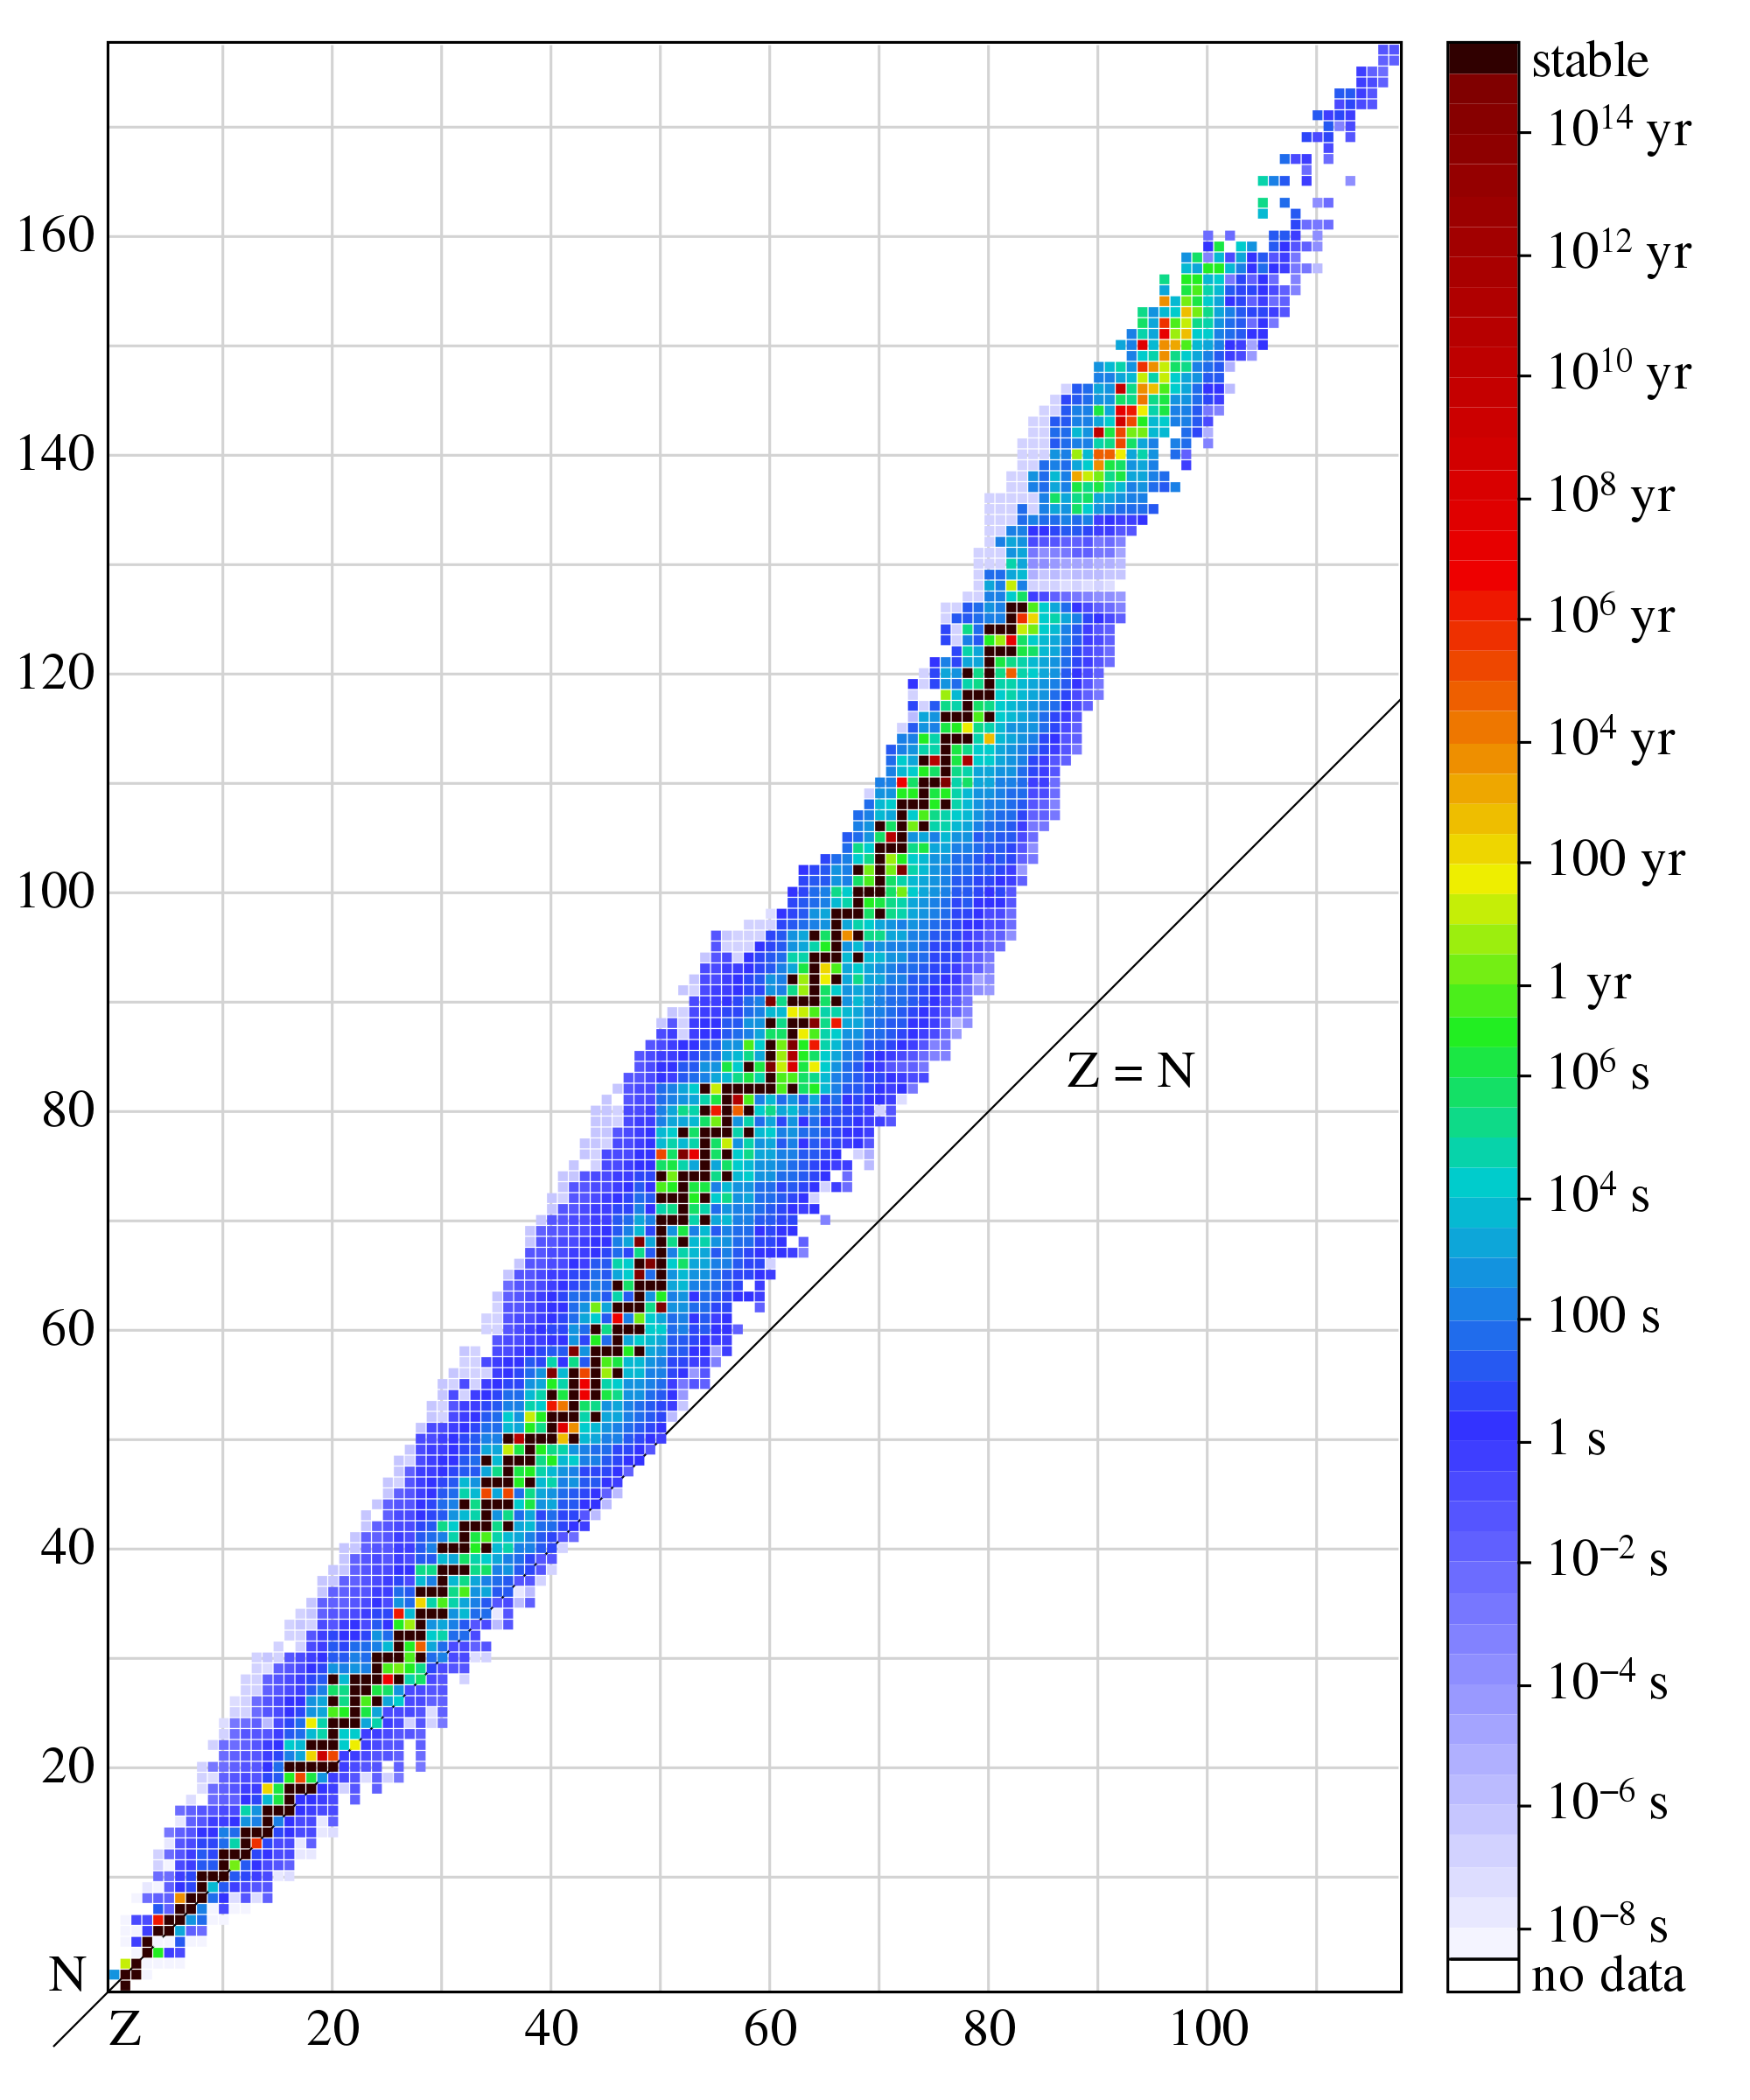
\includegraphics[width=0.8\linewidth]{figures/isotope_halflife} 

}

\caption{Stability of isotopes}\label{fig:halflife}
\end{figure}

\section{Mass Defect}\label{mass-defect}

The mass of an atomic nucleus is less than the sum of the individual
masses of the free constituent protons and neutrons. This ``missing
mass'' is known as the \(\color{Green}{\text{mass\ defect}}\). For
example, the mass defect of a \textsuperscript{12}C atom can be
calculated by:
\[ 6 \times m_p + 6 \times m_n + 6 \times m_e - m_{C} = 0.0988\ amu\]
where \(m_C = 12\) (the ratio of mass to 1 amu). The complete list of
mass number can be found in the
\href{https://physics.nist.gov/cgi-bin/Compositions/stand_alone.pl}{NIST
database}.

The mass defect is closed related to
\(\color{Green}{\text{nuclear binding energy}}\). If we divide the above
energy by 12 and times 931.5 MeV/amu, we obtain the bind energy per
neucleio for \textsuperscript{12}C is 7.67 (see Figure
\ref{fig:stability})

\begin{figure}

{\centering 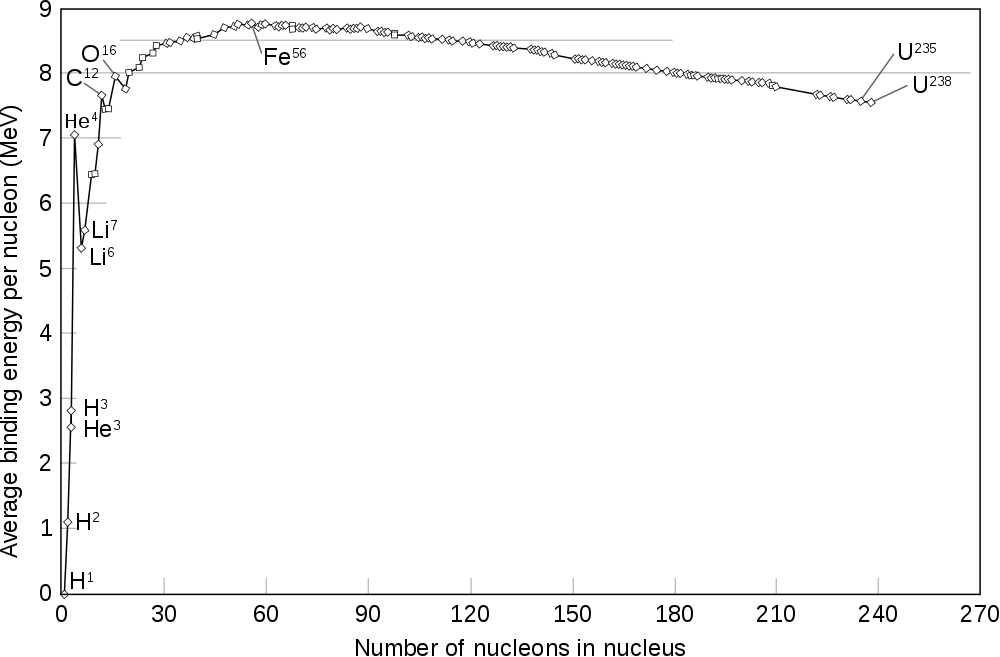
\includegraphics[width=0.8\linewidth]{figures/binding_energy} 

}

\caption{Nuclear binding energy per nucleon (The image is from wiki)}\label{fig:stability}
\end{figure}

A complete table of nuclear bind energies can be found on Lawrence
Berkeley National Laboratory
\href{http://xdb.lbl.gov/Section1/Table_1-1.pdf}{(link)}.

\section{High energy charged particles}\label{einstein}

The mass of a moving particle (not a photon) depends on its velocity
\(\upsilon\) and its rest mass \(m_0\).

\begin{equation}
    E_{total} = mc^2 = \frac{m_0c^2}{\sqrt{1-\frac{\upsilon^2}{c^2}}} 
    \label{eq:emc2}
\end{equation}

or

\begin{equation}
    E_{total} = E_{rest}+E_{K.E} 
\end{equation}

For an electron and a proton accelerated to the velocity of 0.96 c, the
kinetic energy will be about 2 MeV and 2400 MeV. Therefore, high energy
electrons coming out of linac head will have the speed close to the
speed of light. To achieve similar high speed, you need give much more
energy to a proton than an electron.

\section{High energy photons}\label{high-energy-photons}

The energy of a photon is given by

\begin{equation}
    E = h\cdot v
    \label{eq:frequency}
\end{equation}

where h is the Planck constant (\protect\hyperlink{constant}{Physical
constants}), \(v\) is the frequency in unit of
s\textsuperscript{\{-1\}}.

Or

\begin{equation}
    E (eV) = \frac{1.24\times 10^{6}}{\lambda (m)}, 
    \label{eq:wavelength}
\end{equation}

\section{Electron Shell}\label{electron-shell}

\begin{itemize}
\tightlist
\item
  { Principle } quantum number (\(n = 1, 2, 3, ...\) or K, L, M,
  \ldots{}) -- the main energy level (or shell) occupied by an electron.
  The energy can be calculated
  by\[E_n=\frac{Z^2{\hbar}^2}{2m_0\alpha^2_Bn^2},\] where \(\alpha_B\)
  is the \(\color{Green}{\text{bohr radius}}\)
  (\(5.29 \times 10^{-11}m\)). The \textbf{K shell} (binding) energy for
  Lead, Tungsten, and Carbon are 88, 69.5, and 0.28 KeV.
\item
  { Secondary } quantum number (\(l = s, p, d, ...\)) -- the energy
  sublevel (angular monentum) occupied by the electron.
\item
  { Magnetic } quantum number (\(m_l = -l, -l+1, ..., 0, ..., l-1, l\))
  -- the number of possible orientations (projections) for each of
  energy sublevels.
\item
  { Spin } quantum number (\(m_s=-1/2, 1/2\)) -- the two possible
  orientations that an electron can have in the presence of a magnetic
  field.
\end{itemize}

\section{Solutions}\label{solutions}

\texttt{Q1:\ a),\ c),\ (e)} see Section \ref{atomic-rep}\\
\texttt{Q2:\ b),\ d);\ a)\ is\ wrong\ because\ they\ are\ isotopes;\ c)\ is\ wrong\ because\ they\ are\ isobars.}\\
\texttt{Q3:\ a),\ b),\ and\ c)}\\
\texttt{Q5:\ b),\ c);\ a)\ should\ be\ 6\ neutrons\ and\ d)\ should\ be\ 12\ times\ 931\ MeV.}\\
\texttt{Q6:\ see\ above}\\
\texttt{Q7:\ b)}\\
\texttt{Q8:\ d)} see Section \ref{einstein}\\
\texttt{Q9:\ c)}\\
\texttt{Q10:\ a)}\\
\texttt{Q11:\ b)}\\
\texttt{Q12:\ a),\ b),\ c),\ e)}\\
\texttt{Q13:\ b),\ c)}\\
\texttt{Q14:\ c)}\\
\texttt{Q15:\ b)\ using\ Eq.\ \textbackslash{}@ref(eq:wavelength)}
\texttt{Q16:\ c)} using Eq. \eqref{eq:wavelength}

\chapter{Nuclear Transformation}\label{nut}

\begin{quote}
Radioactivity was discoverred in 1986 by A.H. Becquerel when he wa 44
years old (\href{https://en.wikipedia.org/wiki/Henri_Becquerel}{Wiki}).
He received 1903 Nobel Prize in Physics along with Maria and Pierre
Curie.
\end{quote}

\textbf{Radiation Sources} (\href{https://vimeo.com/78875937}{Siebers
2009 AAPM talk}) include

\begin{itemize}
\tightlist
\item
  Radioactive decay (Chapter \ref{nut})

  \begin{itemize}
  \tightlist
  \item
    Alpha-decay
  \item
    Beta-decay (Section \ref{y90})
  \item
    Electron capture
  \item
    Isometric transitions
  \item
    Gamma-ray
  \end{itemize}
\item
  Atomic energy transitions

  \begin{itemize}
  \tightlist
  \item
    Characteristic x-rays
  \item
    Auger electrons
  \end{itemize}
\item
  Accelerated charge particles

  \begin{itemize}
  \tightlist
  \item
    Direct (electrons, protons)
  \item
    x-ray generators (synchrotron radiation (magnetic field),
    Bremmstrahlung)
  \end{itemize}
\item
  Interaction products (?)
\end{itemize}

\section{Decay (disintegration)}\label{decays}

General balance equations of radioactive decay

\begin{equation}
 _Z^A P = ^{A-A_R}_{Z-Z_R}D + _{Z_R}^{A_R}R + \sum Q, 
\end{equation}

where P and D stand for parent and daughter element, R for radiation,
and Q is reaction energy (\(\sum Q = M_P-M_D-M_R\)). To find out the
Q-value, you can use a online
\href{http://www.nndc.bnl.gov/qcalc/}{Q-calculator}.

Atoms found in nature are either stable or unstable. An atom is unstable
(radioactive) if these forces are unbalanced if the nucleus has an
excess of internal energy
\href{http://www.epa.gov/radiation/understand/radiation.html}{EPA link}.
The instability of a radionuclide may result from an excess of either
neutrons or protons. Radionuclides attempt to reach stability through

\begin{enumerate}
\def\labelenumi{\arabic{enumi}.}
\tightlist
\item
  ejecting neutrons and protons (C area; Alpha-decay);
\item
  converting one to the other with ejection of a beta particle or
  positron (B area; Beta decay);
\item
  the release of additional energy by photon emission (Gamma decay).
\end{enumerate}

\subsection{Alpha-decay}\label{alpha}

Alpha-decay occurs in nuclides with atomic numbers above 82 (only the
first 92 occur naturally) and where the ratio of neutrons to protons is
low, thus resulting in the repulsive coulomb force of the protons
overcoming the attractive strong nuclear force.

\[
\begin{matrix}
\underline{\text{Example}} & _{88}^{226}Ra\rightarrow _{86}^{222}Rn +_2^4\alpha +\gamma +Q
\end{matrix}
\]

\subsection{Beta-decay}\label{beta}

Beta-decay, a neutron within the nucleus is converted into a proton, and
an electron and an antineutrino are emitted, or a proton is converted
into a neutron, and a positron and a neutrino are emitted. The forces
responsible for the \(\beta\)-decay are weak (referred to as \emph{weak
nuclear force}) compared with both the strong nuclear force and the
electrostatic force among the nucleons.

\[
\begin{matrix}
\underline{\text{Example}} & \begin{matrix}
    \beta^-\  \text{decay}& _{60}^{27}Co\rightarrow _{27}^{60}Ni^{*} +\beta^- + \bar\nu \\ 
    \beta^+\  \text{decay} & _{9}^{18}F\rightarrow _{8}^{18}O +\beta^+ +\nu + 1.022\ \text{MeV}
  \end{matrix}
\end{matrix}
\]

\emph{Neutrino} (\(\nu\)) and \emph{anti-neutrino} (\(\bar \nu\))
results in spectrum of \(\beta\) energies, and they are non-ionizing
particles so we don't consider them in dose calculation.

\subsection{Electron capture}\label{ec}

Electron capture (EC) is an alternative to positron decay. In this
process, an electron, usually in the K shell, is captured within the
nucleus and combined with a proton to create a neutron. Electron capture
most often is followed by characteristic x-ray or Auger electron.

\subsection{Gamma decay}\label{gamma}

Gamma decay occurs when a nucleus undergoes a transition from a higher
to a lower energy level. These \(\gamma\)-rays are identical to the
x-rays emitted by excited atoms, except that \(\gamma\)-rays originate
from within the nucleus and x-rays originate from outside the nucleus.

\[
\begin{matrix}
\underline{\text{Example}} & _{27}^{60}Ni^{*} \text{ decay to stable }_{27}^{60}Ni \text{ by emitting two } \gamma \text{-rays with energies of 1.17 and 1.33 MeV.}
\end{matrix}
\]

The decay scheme can be found
\href{http://atom.kaeri.re.kr:8080/gamrays.html}{here}.

\section{Activity}\label{activity}

The \texttt{activity} (A) of a sample is the average number of
disintegrations (decay) per second,

\begin{equation}
A = \frac{\Delta N}{\Delta t} = \lambda N,
\end{equation}

where \(\lambda\) is the \texttt{decay\ constant} which is the
probability that a nucleus will decay per second. Remember that
Radioactive decay is a \textbf{stochastic} process. We can find certain
laws only by observing a large number of events (decays here).

From the equation above, we can obtain the radioative decay law at a
certain time \(t\):

\begin{equation}
N = N_0 e^{-\lambda t},
\label{eq:decay1}
\end{equation}

or

\begin{equation}
A = A_0 e^{-\lambda t}. 
\label{eq:decay2}
\end{equation}

More frequently, we use \texttt{half-life\ time} (\(T_{1/2}\)) instead
of the decay constant \(\lambda\). Their reqlationship is

\begin{equation}
  T_{1/2} = \frac{\ln 2}{\lambda}.
  \label{eq:halflife}
\end{equation}

The \emph{mean} or \emph{average} life is the (arithmetic) average
lifetime for the decay of radioactive atomes.

\begin{equation}
  T_{a} \equiv \frac{1}{\lambda} = 1.44T_{1/2}.
    \label{eq:avelife}
\end{equation}

\section{Unit}\label{decay-unit}

The SI unit for radioactivity is \emph{Becquerel} (Bq). The historic
unit for radioactivity is Curie (Ci), and 1g of radium is 1 Ci. The
relationship between Curie and Becquerrel is

\begin{equation}
 1\ Ci = 3.7 \times 10^{10} \ Bq
 \label{eq:curie2bq}
\end{equation}

In practice, the more frequently used formula is

\begin{equation}
  \bold {1\ \text{GBq} = 27\ \text{mCi}}
\end{equation}

\section{Solutions}\label{nucl-solution}

\textbf{Q1 Decays}

Using Eq. \eqref{eq:decay1} or \eqref{eq:decay2} and \eqref{eq:halflife}, we
get

\[
\text{Residual activity} = 1-0.02 = e^{-\frac{ln2}{30}t} \rightarrow \boxed{t =0.87\ \text{years}}
\]

It is easy to solve the above equation, but it will be faster to find a
good estimation using the \texttt{Taylor’s\ expansion} with first two
terms \(e^{-\frac{ln2}{30}t} \approx 1-\frac{0.693}{30}t\). The caveat
of using Taylor expansion is make sure the exponents are much smaller
than 1. You can try this approach for question 3, but you will not get
the correct answer.

\texttt{Q2\ b),\ e)}\\
\texttt{Q4\ a)\ b)}\\
\texttt{Q5\ c)}\\
\textbf{Q6 Calculation of total decay}

\[
\begin{aligned}
\text{Decay}_{total} &= 1.44 \times T_{1/2} \times {A} \\
    &= 1.44 \times 30 \times 3.15\times 10^7 \times 3.7\times 10^9 \\
    &= \boxed{5.04\times 10^{18}}
\end{aligned}
\] \textbf{Q6 Average life time} \[
A=A_0e^{-\lambda T_a}=A_0e^{-\lambda \frac{1}{\lambda}}\rightarrow \frac{A}{A_0}=e^{-1} \approx \boxed{37\%}
\] For question 6, with 1 year = 31536000 s and Eq. \eqref{eq:curie2bq},
the total number of decays is equalt to total activity of 10 mCi Cs-137
is \[
10e^{-\frac{0.693}{8.05}t} = 4e^{-\frac{0.693}{14.3}t} \xrightarrow{\text{take ln() on each side}}
  ln10-\frac{0.693}{8.05}t = ln4 -\frac{0.693}{14.3}t \rightarrow t = \boxed{24.3\ \text{days}}
\]

\textbf{Q7} c)

\textbf{Q8}

b); For higher electrons coming out of linac head, the electron velocity
is close to the speed of light.\texttt{}Q9 a)\texttt{}Q10 b)\texttt{}Q11
d)\texttt{}Q12 b) d)\texttt{}Q13 c)`

\chapter{Production of X-rays}\label{prox}

\section{History}\label{history}

\begin{itemize}
\tightlist
\item
  Cathod-ray tube (for example, Crookes tube)\footnote{partially vaccum
    and low voltage; think about neon lighting; see
    \href{https://en.wikipedia.org/wiki/Crookes_tube}{wiki}}.
\item
  1895-11-08, Wilhelm Rontgen discovered x-ray by observing fluorsece
  when applying high volotage (using an induction coil) on a
  board-covered Crookes tube
  (\href{https://en.wikipedia.org/wiki/Wilhelm_Röntgen}{wiki} and
  \href{https://www.youtube.com/watch?v=qVn3mgt8Two}{The Laureates:
  William Roentgen}.
\item
  Coolidge developed the \textbf{hot cathode} x-ray tube in 1913, in
  which a wire filament was heated with electrical current to release
  electrons by the process of \texttt{thermionic\ emission}. This was
  the first major breakthrough as cathod-ray tubes cannot generate
  reliable and high-intensity x-ray.
\item
  The next major breakthrough in x-ray tube design was the
  \textbf{rotating anode}, which was developed by Albert Bouwers in
  1930.
\end{itemize}

\begin{figure}
\centering
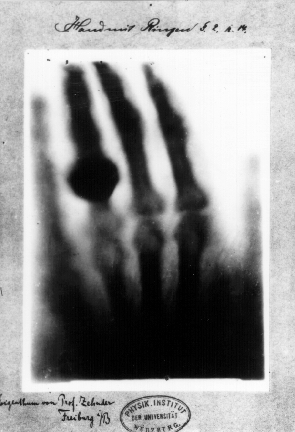
\includegraphics{figures/x-ray_hand.jpg}
\caption{First medical X-ray by Wilhelm Röntgen of his wife Anna Bertha
Ludwig's hand. (The image is from
\href{https://en.wikipedia.org/wiki/Wilhelm_Röntgen}{wiki})}
\end{figure}

\begin{quote}
\textbf{The Coolidge tube was the prototype for x-ray tubes in use
today.}
\end{quote}

\section{Conventional x-ray tubes}\label{conventional-x-ray-tubes}

The basic components of a useful x-ray tube include: (a) electron
source, (b) high voltage supply, (c) target for x-ray production, (d)
vacuum, and (e) collimator.

\subsection{Electron Source}\label{electron-source}

\begin{itemize}
\tightlist
\item
  Tungsten (melting point is 3370 \textsuperscript{o}C).
\item
  The filament is housed within a negatively charged focusing cup.
\item
  With high voltage applied across the tube, thermonic electrons are
  attracted to the target (anode) without electrons pile-up around the
  filement. In this scenerio, the tube is operated in the mode of
  \texttt{filament-emission\ limited}.
\item
  With lower voltage applied across the tube, thermonic electrons are
  not pulled immediately to the target. The accumulated electrons
  (\emph{space charge}) will prevent additional electrons leaving the
  filament and therefor limit the tube current. Under this condition,
  the tube is operated in the mode of \texttt{space-charge\ limited}
  (e.g.~mammography machine).
\item
  Dual-focus x-ray tube
\end{itemize}

\subsection{High voltage}\label{high-voltage}

The electric potential difference (voltage) between the filament
(cathode) and target (anode) of an x-ray tube affects the x-ray output,
\textbf{intensity} (see electron source part) and spectrum of x-ray.

high-frequency x-ray generators (1-100 kHz)

kVp: maximum or peak volotage

\texttt{Applications}

\begin{itemize}
\tightlist
\item
  CT-simulator
\item
  kV-CBCT
\end{itemize}

\section{X-ray spectra}\label{x-ray-spectra}

`The efficience is

\chapter{Clinical Treatment Generators}\label{gene}

\section{History}\label{history-1}

\begin{itemize}
\tightlist
\item
  \texttt{Cyclotron} Earnest O. Lawrence 1932
\item
  \texttt{Betatron} Donald W. Kerst 1940
\item
  \texttt{Cobalt\ machine}
\item
  \texttt{Linear\ accelerator} 1950s
\item
  \texttt{Gamma\ knife} Lars Leksell 1968
\end{itemize}

\section{Waveguide}\label{waveguide}

\begin{figure}

{\centering 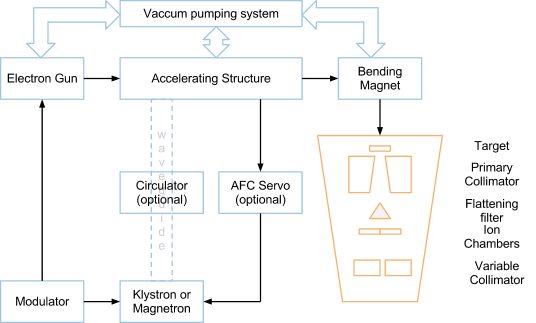
\includegraphics{figures/components} 

}

\caption{a simple schematic of a linear accelerator}\label{fig:unnamed-chunk-3}
\end{figure}

\section{Microwave amplifier}\label{microwave-amplifier}

The possibly best simple explanation about how a
\href{https://www.youtube.com/watch?v=Fvud81pYGOg}{klystron} amplifier
and \href{https://www.youtube.com/watch?v=VkpEQZEGSkE\&t=108s}{microwave
oscillators} work can be found on YouTube.

A \texttt{Klystron} is a microwave (300 MHz -- 300 GHz) amplifier tube
that makes use of two (or more for better bunching result) resonant
cavities. For a simple two cavity Klystron,

\begin{enumerate}
\def\labelenumi{\arabic{enumi}.}
\tightlist
\item
  The first resonance cavity is energized by very low-power microwaves
  through a coaxial cable.
\item
  The microwave will cause alternating ``E'' fields across the gap
  between left and right cavity wall.
\item
  As the electrons from the accelerated through the first cavity, half
  of them will be decelerated and the other help will accelerate
  (velocity modulation), and thus form electron bunches as they drift
  towards the second cavity.
\item
  The Catcher cavity is resonant at the arrival frequency of the bunch.
\item
  This will generates a retarding ``E'' field for slowing down electrons
  and in turn the electrons give their energies in the form of
  high-power microwaves (more electrons in a bunch \(\rightarrow\) more
  kinetic energy \(\rightarrow\) more EM energies induced in the 2nd
  resonant cavity).
\end{enumerate}

\begin{figure}

{\centering 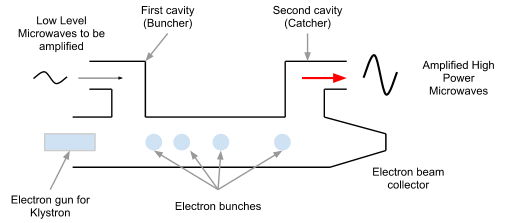
\includegraphics{figures/klystron} 

}

\caption{how a klystron works}\label{fig:unnamed-chunk-4}
\end{figure}

A \texttt{Magnetron} is a device that produces microwaves.

\begin{enumerate}
\def\labelenumi{\arabic{enumi}.}
\tightlist
\item
  The electrons emitted from the heated cathode are accelerated by the
  pulse electric field, EP, toward the anode across the evacuated drift
  space between cathode and anode.
\item
  A static magnetic field, H, is applied perpendicular to the cross
  section of the device.
\item
  The accelerated electrons induce an additional charge distribution
  shown on the anode poles and an electric field Em of microwave
  frequency between adjacent segments of the anode (similar to that in
  the catcher cavity of the klystron).
\end{enumerate}

\begin{figure}

{\centering 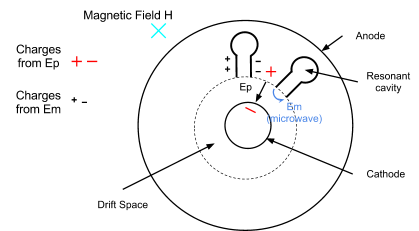
\includegraphics{figures/magnetron} 

}

\caption{how a magnetron works}\label{fig:unnamed-chunk-5}
\end{figure}

\section{Microwave frequency}\label{microwave-frequency}

The microwave pulse frequency in most medical linear accelerators is
about \textbf{3 GHz}, which falls into the category of IEEE
\texttt{S-band} (2-4 GHz, Wiki). The Mobetron and Cyberknife machines
use higher frequency (8-12 GHz, categorized as in IEEE \texttt{X\ band},
for compact design (Hanna 1999
\href{https://accelconf.web.cern.ch/AccelConf/p99/PAPERS/WEP114.PDF}{Applications
of X-band Technology in medical accelerators}).

\section{Penumbra}\label{penumbra}

The term \texttt{Penumbra} means the region, at the edge of a radiation
beam, over which the dose rate changes rapidly as function of lateral
distance. The overall penumbra was contributed from three sources:

\begin{itemize}
\tightlist
\item
  \emph{Geometric penumbra} is caused by the source (or focal spot)
  having a finite size and the location of the collimator. It can be
  reduced by decreasing the focal spot and move the collimator closer to
  the patient (e.g.~Varian tertiary MLC).
\item
  \emph{Transmission penumbra} is caused by photons transmitted through
  the edge of the collimator. It can be reduced by aligning the
  collimator following the beam divergence (e.g.~X and Y photon jaws).
\item
  \emph{Physical (total) penumbra} is the combination of transmission,
  geometric penumbra, and lateral scatter of radiation (photon and
  electrons) within the patient. Lateral electron disequilibrium (\# of
  electrons projected laterally outward is not equal to \# of electrons
  projected laterally inward). Because the range of these laterally
  projected electrons increases as energy increases, higher energy beams
  have a slightly greater penumbra than low energy beams.
\end{itemize}

\chapter{Interaction}\label{inter}

\begin{quote}
Follow the energy
\end{quote}

\section{Photoelectric interactions}\label{photo-el}

The probability\footnote{The basic quantity in collisional dynamics is
  \texttt{cross\ section}. The SI unit is \(cm^2\) and the unit is
  \texttt{barn} (\(1\ b = 10^{-24}\ cm^2\)) in nuclear physics.} of
\emph{photoelectric interaction} \(\propto\)
\(\color{blue} {\frac{Z^3}{E^3}}\).

\begin{itemize}
\tightlist
\item
  incident photon interact with bound atomic electron;
\item
  \textbf{all energy} is given to electron;
\item
  an orbital electron is ejected possessing most of incident photon, and
  a vacancy is present;
\item
  Characteristic x-ray and \emph{Auger} electron (The energy released by
  the downward transition is given to one of the outer electrons instead
  of to a photon).
\end{itemize}

\section{Compton interactions}\label{compton}

The probability of \emph{Compton interaction} \(\propto\)
\(\color{blue} {\rho_e}\).

\begin{itemize}
\tightlist
\item
  interaction between incident high energy photons and loosely bound
  orbital electrons.
\item
  With \(\alpha = \frac{hv_0}{m_ec^2}\) and \(\theta\) is the angle
  between incident and scattered photon, the scattered photon energy is

  \begin{equation*}
    E_p = hv_0\frac{1}{1+\alpha(1-\cos\theta)}.
  \end{equation*}

  \begin{enumerate}
  \def\labelenumi{\alph{enumi}.}
  \tightlist
  \item
    with \(\theta = 0^o\) (glazing hit) electron acquires minimum
    energy, \(\Delta\lambda = .00243\times(1-\cos\theta)\);
  \item
    with \(\theta = 90^o\) for megavoltage linacs with \(\alpha\)
    \textgreater{} 10, scatter photons always have energy of about 0.5
    MeV (shielding consideration);
  \item
    with \(\theta = 180^o\) (photon is scattered back) electron acquires
    maximum K.E and photon has an energy of 0.255 MeV.
  \end{enumerate}
\end{itemize}

\texttt{Q2:\ d)}

\section{Pair production}\label{pair}

The probability of \texttt{pair\ production} \(\propto\)
\(\color{blue} {Z\cdot E}\).

\begin{itemize}
\tightlist
\item
  occurs when a photon approaches closely enough to the target nucleus;
\item
  the incident photon energy may be converted directly into an
  electron-positron pair. When the positron comes to rest, it combines
  with an electron, and both particles then undergo annihilation, with
  the appearance of two photons with energy of 0.511 MeV traveling in
  opposite directions.
\end{itemize}

\texttt{Q3:\ b)\ The\ threshold\ energy\ for\ pair\ production\ is\ 1.022\ MeV.}

\section{Compton interactions}\label{compton-interactions}

If the photon is scatter back at \(\theta = 180^o\), the electron gains
the maximum energy \(hv \times \frac{2\alpha}{1+2\alpha}\).

\begin{equation}
    \lambda'-\lambda = \frac{h}{mc^2}(1-cos\theta)
\end{equation}

\textbf{Attenuation} of radiation is removal of photons or energy from a
beam by different interactions including absorption and scatter. Like
the process of radioactive decay, the attenuation is also a stochastic
process

For a thin absorber, with absorber far away from the source (so effect
of beam divergence is negligible e.g.~ignore inverse square
law\footnote{The intensity of a point radiation source follows inverse
  square law. This a kind of geometric concept as the area of a sphere
  is \(A = 4\pi r^2\). The inverse square law is valid under two
  assumptions: (1) point source, i.e.~small enough compare to distance;
  (2) photon undergoes no interaction (e.g.~TBI with spoiler).}), or in
a \textbf{narrow} beam geometry, we get \(-\Delta N/N = \mu \Delta x\),
where \(\mu\) is \texttt{linear\ attenuation\ coefficient} which can be
thought as the fraction of photons or energy removed from beam per cm of
absorber beam per cm. Half-value layer (HVL) relates to the linear
attenuation coefficient by

\begin{equation}
    HVL = \frac{0.693}{\mu}
\end{equation}

\emph{Mass attenuation coefficient} is often used to remove the
dependence of the physical density.

\begin{equation}
\left(\frac{\mu}{\rho}\right) \propto \frac{\sigma_{tot}}{\rho} =                       \frac{\sigma_{coh}}{\rho}+\frac{\sigma_{pe}}{\rho}+\frac{\sigma_{comp}}{\rho} + 
\frac{\sigma_{pair}}{\rho} + \frac{\sigma_{trip}}{\rho} + \frac{\sigma_{ph.n}}{\rho}
\end{equation}

\chapter{Measurement of Ionizing Radiation}\label{measurement}

Attempts were made to measure ionizing radiation based on chemical
and/or biological (skin) effects. But those measurements were not
reliable. The ICRU adopted the roentgen, denoted by R, as the unit of
measuring x- and \(\gamma\)-ray exposure.

The
\href{https://onlinelibrary.wiley.com/doi/abs/10.1002/jlcr.2580180918}{ICRU
No.33 (1980)} (1980) definition of exposure: \[X=\frac{dQ}{dm},\] where
dQ is the absolute value of the total charge of the ions of one sign
produced in air when all the electrons (negatrons and positrons)
liberated by photons in air of mass dm are completely stopped in air.

From the book ``Fundamentals of Radiation Dosimetry'' (chapter 5 - good
chapter to read): the photons first interact with a defined mass of air.
They will produce electrons by the photoelectric and Compton effect and
both electrons and positrons by the pair production process. All those
secondary charged particles must travel through the air until their
energy is

\section{Collection volume}\label{collection-volume}

A free air ionization chamber has a 10 mm diameter aperture, a plate
separation of 90 mm, and a collection length of 70 mm. Calculate the
mass of air in the collection region.
\[ mass = \rho \cdot V = 1.293\ kg/m^3 \cdot \frac{1}{4}\pi\times(10\ mm)^2\times 70\ mm = 2.3\times10^{-7} kg\]

\section{Signal of an ion chamber}\label{signal-of-an-ion-chamber}

The signal from an ionization chamber is proportional to the charge
(ionization) collected (so to the numbers of gas molecules in the
cavity. Combining the ideal gas law (\(P \cdot V = nRT\)), we have
\[signal \propto \frac{P \cdot V}{T} \]

In this case, \(V_{unsealed}=(1/2)^3 V_{sealed}\) and P\_unsealed = 1atm
= 1/3 P\textsubscript{sealed}.

\section{Temperature and pressure
correction}\label{temperature-and-pressure-correction}

Most likely, the local measurement condition will be different from the
standard environment condition (\(22^{o}C\) and 760 mmHg) under which
the ion chamber (and possible its electrometer) is calibrated. Therefore
we need to correct the reading with a factor (AAPM TG-51):

\begin{equation}
  P_{TP}=\frac{(237.2+T)}{(273.2+22.0)}\times\frac{760}{P},
  \label{eq:ptp}
\end{equation}

wehre T is in the unit Celsus and P is in the unit of mmHg.

\begin{quote}
Pressure drops about 1 inch per 1000 feet.
\end{quote}

So the pressure is 760 -- 3600/1000 x 25.4 = 668.6 mmHg.
\(P_{TP}=\frac{273.2+24}{273.2+22.0} \times \frac{760}{668.6}=1.14\)
\(P_{TP_wrong}=\frac{273.2+24}{273.2+22.0} \times \frac{760}{760}=1.006\);
If we used the wrong P\_\{TP\}, the ``corrected'' reading (machine
output) will be thought as 13\% lower than the actual value. If we
increase linac output to compensate this 13\% difference, we will
overdose the patient by 13\%.

\texttt{Q6:\ a);\ Q7:\ d);\ Q8:\ d);\ Q9:\ b)}

\begin{verbatim}
C); but this is different from my calculation! The plate separation of 90 mm is not used here.
E)
\end{verbatim}

Chp6 c c d e b a d d b b d bcd b bc acd

\href{https://www.aapm.org/meetings/09SS/documents/05Seuntjens-MonteCarloIntro.pdf}{Rogers's
talk}

\section{Guard electrode}\label{guard-electrode}

The guard electrode in a Farmer-type chamber can (1) prevent leakage
from the high-voltage collector electrode; (2) define the ion-collecting
volume; and (3) minimize polarity effect (?).

\texttt{a),\ c),\ d)}

Good reading materials include Deward A good document can be found here.

Figure Radiographs (above) and drawings (below) of five
Baldwin--Farmer-style ion chambers plus an Exradin A12 . In the
drawings, the heavy black lines represent the extent of guarding, as
also indicated by the arrows on the left. The grey blocks indicate the
insulator in closest contact with the active air volume, indicated by
the arrows on the right. The A12 has no insulator other than air in
contact with the active air volume. (PMB 50 N121, 2005)

\chapter{Quality of X-rays}\label{quality}

We have finished a nice book.

\chapter{Absorbed Dose}\label{dose}

\begin{quote}
``Perhaps one of the greatest contributions physics has made to
radiation oncology and radiology, x-ray imaging and all of its forms has
been in developing ways to measure radiation accurately and precisely
(commonly `using ion chamber).''

--- Peter Almond
\end{quote}

To measure the absorbed dose from ionizing radiation within a medium, we
need to know

\begin{enumerate}
\def\labelenumi{\arabic{enumi}.}
\tightlist
\item
  The number of particles or photons, or the quantity of energy, passing
  through the medium (\emph{fluence})
\item
  The quantity of energy transferred from initial particles (often
  photons, which are uncharged) to charged particles in the medium
  (\emph{KERMA})
\item
  The rate at which energy is transferred from the charged particles in
  the medium, to the medium itself (stopping power, leading to absorbed
  dose).
\end{enumerate}

\(\color{Green}{\text{Fluence}}\) is defined as the number of particles
\(dN\) incident on a sphere of cross-sectional area \(da\). The SI unit
is \(m^{-2}\)

\begin{equation}
    \Phi = \frac{dN}{da}
    \label{eq:fluence}
\end{equation}

\(\color{Green}{Energy\ fluence}\) (\(\Psi\), unit: \(J\cdot m^{-2}\))
is defined as the energy dE incident on a sphere of cross-sectional area
da. The SI unit is \(J\cdot m^{-2}\).

\begin{equation}
    \Psi = \frac{dE}{da}
    \label{eq:efluence}
\end{equation}

If you have a fluence \(\Phi\) of particles all of energy E, then the
energy fluence is simply \(\Psi = \Phi\cdot E\).

\(\color{Green}{KERMA}\) (Kinetic Energy Released per unit MAss) is
defined as the mean kinetic energy transferred to charged particles from
uncharged particles in a mass dm of a given material. The SI unit is
J/kg, and the special name for the unit for Kerma is gray (Gy).

\begin{equation}
    K=\frac{d\bar E_{tr}}{dm} ~ (J\cdot kg^{-1}\ or\ Gy)
    \label{eq:kerma}
\end{equation}

The relation between Kerma and fluence can be expressed as
\[K=\int \Psi(E)\frac{\mu_{tr}(E)}{\rho}dE\] Where
\(\frac{\mu_{tr}(E)}{\rho}\) is the mass energy transfer coefficient of
the material for uncharged particles of energy E.

\(\color{Green}{Unrestricted\ stopping\ power}\) for charged particles
(electrons) is defined as \[ S = \frac{dE}{dx} \]

\begin{itemize}
\tightlist
\item
  Collisional stopping power (\(S_{coll}\))
\item
  Radiative stopping power (\(S_{rad}\)) -- cause by the interactions of
  charged particles with nuclear electric field -- bremsstrahlung
  radiation The relationship of fluence and stopping power to absorbed
  dose is given by:
\end{itemize}

\[D_{med}=\int \Phi_{med, E}(E)\frac{S_{coll}(E)}{\rho}dE\]

\section{Optical density}\label{optical-density}

The details about the radiographic films can be found in AAPM
\href{https://www.aapm.org/pubs/reports/RPT_216.pdf}{TG-69}:
Radiographic film for megavoltage beam dosimetry.

\section{Q9 OD}\label{q9-od}

A pivotal assumption in film dosimetry is that the dose to the film is
reflected in the resulting ``blackness'' or optical density (OD) of that
film.\\
\[OD=log_{10}\left( \frac{1}{T}\right)=log_{10}\left( \frac{I_0}{I_t}\right)\]

The details about radiochromic films can be found in AAPM
\href{http://www.aapm.org/pubs/reports/RPT_216.pdf}{TG-55} and its
update AAPM
\href{http://www.aapm.org/org/structure/default.asp?committee_code=TG235}{TG-235}
as well an excellent review article by
\href{http://hepweb03.phys.sinica.edu.tw/opto/Irradiation/RadioChromic/Documents/MSE41_61.pdf}{Butson
et al. ``Radiochromic film for medical radiation dosimetry'' (2003)}.
Table 1 lists the radiation interaction processes and their variation
with Z.

Relative dosimeter

\begin{itemize}
\tightlist
\item
  Diode (single or 2D diode array MapCheck)
\item
  TLD
\item
  OSL
\item
  MOSFET
\item
  Film
\end{itemize}

\chapter{Dose Distributions}\label{distribution}

\section{TAR}\label{tar}

The first three factors are used for the source-to-axis distance (SAD)
technique (mechanical isocenter and radiation isocenter roughly
coincidence with the tumor centroid).

With \(d\) is the depth from the surface to the isocenter in a phantom
and \(r\) is the field size at the level of the isocenter, we can define

\begin{itemize}
\tightlist
\item
  \texttt{Tissue-air-ratio} (TAR) is defined by
\end{itemize}

\begin{equation}
  TAR(d,r_d) = \frac{Dose_{phantom}(d)}{Dose_{air}}
  \label{eq:tar}
\end{equation}

\begin{itemize}
\tightlist
\item
  \texttt{Backscatter\ factor} (BSF) is a special case of TAR, in which
  \(d=d_max\)
\end{itemize}

\begin{equation}
  BSF = \frac{Dose_{phantom}(d_max)}{Dose_{air}}
  \label{eq:bsf}
\end{equation}

\begin{itemize}
\tightlist
\item
  \texttt{Scatter-air\ factor} (SAR) can be calculated by
\end{itemize}

\begin{equation}
  SAR(d,r) = TAR(d,r)-TAR(d,0)
  \label{eq:sar}
\end{equation}

THe \texttt{Mayneord\ factor} is used to find a new PDD from a known PDD
value

\begin{equation}
  f = \frac{PDD_2}{PDD_1} =\left( \frac{SSD_2+d_{max}}{SSD_1+d_{max}} \right)^2  \cdot \left( \frac{SSD_1+d}{SSD_2+d} \right)^2  
  \label{eq:mayneord}
\end{equation}

\chapter{Dose calcuation}\label{dosecalc}

We have finished a nice book.

\chapter{Treatment Planning I: Isodose Distribution and Plan
Evaluation}\label{planning1}

\section{Penumbra}\label{penumbra-1}

The dose distribution outside the field boundaries is significantly
affected by geometric penumbra, depth, leakage radiation through
collimator. The flattening filter mostly affect dose within the field
boundary.

\section{Wedges}\label{wedges}

\begin{itemize}
\tightlist
\item
  Physical wedge

  \begin{itemize}
  \tightlist
  \item
    External physical wedge
  \item
    Internal physical wedge (aka motorized wedge, as in
    Elekta\textsuperscript{TM} machines) typically consists of a single
    large wedge (e.g., 60 degrees) placed above the secondary
    collimating jaws. The smaller angle is form by combining the open
    (o) field and the 60\(^o\) degree wedge field:
    \[ Dose_{\theta}=W_{o}Dose_{o} + W_{60^o}Dose_{60^o},\] where
    \(W_{60^o}=\frac{tan\theta}{tan{60^o}}\).
  \end{itemize}
\item
  Non-physical wedge

  \begin{itemize}
  \tightlist
  \item
    \emph{Virtual wedge} (as in Siemens\textsuperscript{TM})
  \item
    \emph{Enhanced dynamic wedge} (EDW) in Varian\textsuperscript{TM},
    which is implemented by moving one of the collimating jaws from one
    end of the field to the other.
  \end{itemize}
\end{itemize}

\emph{Wedge (isodose) angle} is defined as the angle between wedged
isodose curve (see figure wedge isodose) and the normal to the central
axis at a specific depth (e.g., 10 cm). What we typically measure is
wedge profile.

\textbf{Wedge Commissioning}

\begin{itemize}
\tightlist
\item
  \href{http://www.uni-ulm.de/~jsalk/edw/edw.pdf}{Salk et al} Physical
  aspects in the clinical implementation of the EDW - \textbf{1D ion
  chamber}.
\item
  \href{https://www.ncbi.nlm.nih.gov/pubmed/19928081}{Fontanarosa et al}
  Commissioning Varian EDW in the PINNACLE treatment planning system
  using \textbf{Gafchromic EBT film}.
\item
  \href{http://onlinelibrary.wiley.com/doi/10.1120/jacmp.v16i5.5498/full}{Njeh}
  EDW output factors for Varian 2300 CD and the case for a reference
  database.
\item
  Shao et al the accuracy of dynamic dose computation in the ADAC
  Pinnacle RTP system.
\item
  \href{http://onlinelibrary.wiley.com/doi/10.1118/1.598019/epdf}{Zhu et
  al} Performance evaluation of a diode array for EDW dosimetry -
  \textbf{mapcheck}.
\item
  \href{http://www.jmp.org.in/article.asp?issn=0971-6203;year=2010;volume=35;issue=1;spage=33;epage=41;aulast=Ahmad}{Ahmad
  et al} Study wedge factors and beam profiles for physical and EDW
\end{itemize}

\chapter{Treatment Planning II: Patient Data, Corrections, and
Setup}\label{planning2}

\section{Inhomogeneity}\label{inhomogeneity}

In the presence of inhomogeneity, the dose calculation needs to address
two issues
(\url{https://www.utoledo.edu/med/depts/radther/pdf/JC\%20Chapter\%2011\%20handout.pdf}):

\begin{enumerate}
\def\labelenumi{\arabic{enumi}.}
\tightlist
\item
  Change in primary fluence (see Eq. \eqref{eq:fluence}) due to change in
  attenuation
\item
  Change in scatter contributions.
\end{enumerate}

calculation either indirectly through a correction factor (CF) or
directly inherent in the algorithm (Papanikolaou AAPM presentation)

\section{Range}\label{range}

The energy loss of electrons in a medium can be evaluated using
\texttt{mass\ stopping\ power} (\(S/\rho\)) in unit of
\(\frac{MeV}{g\cdot cm^2}\)

\[
\begin{aligned}
\left(\frac{S}{\rho}\right) 
&=\left(\frac{S}{\rho} \right)_c +\left(\frac{S}{\rho} \right)_r \\
&=\frac{\frac{dE}{dl}} {\rho}
\end{aligned}
\]

The detailed information about stopping power for electrons can be found
on the NIST website
(\url{https://www.nist.gov/pml/stopping-power-range-tables-electrons-protons-and-helium-ions}).

In the range of therapeutic energies, 4 MeV to 20 MeV, the total`mass
stopping power is almost a constant, e.g.,

\begin{equation}
  \color{Blue} {\left(\frac{S}{\rho}\right) \approx 2 \frac{MeV\cdot {cm}^2}{g}}
  \label{eq:stopping}
\end{equation}

For water, the \texttt{stopping\ power} (S) is equal to
\(S = \left(\frac{S}{\rho}\right) \times \rho \approx 2 \frac{MeV\cdot {cm}^2}{g}\times 1 \frac{g}{cm^3} = 2 \frac{MeV}{cm}\).

For an electron beam of energy E, which is specified as the most
probable energy at the surface \((E_P)_0\), the practical range of a
broad electron beam in water can be estimated by \(R_P = E/12MeV\).

\section{MRI}\label{mri}

\href{https://www.youtube.com/watch?v=zf5oX01bRgk\&t=1147s}{Shimony's
Youtube video} and more resources at 2:41.

\textbf{Basics}

\begin{enumerate}
\def\labelenumi{\arabic{enumi}.}
\tightlist
\item
  A strong, uniform magnetic field \(B_0\)\footnote{For a simple long
    solenoid with uniform winding density, the magnetic field will be
    \[ B= \mu_0IN/L,\] where B is field strength, \(\mu_0\) is the
    \href{https://en.wikipedia.org/wiki/Permeability_(electromagnetism)}{permeability}
    constant of free space (\(1.27 \times 10^{-6} mks^{-2}A^{-2}\);
    about the same as those for water, hydrogen, and human body), I is
    current per turn, N is the number of turns, L is the coil length.
    For B = 1 T, L = 1 m, N = 10,000, the current will be around 80 A
    \href{https://www.europhysicsnews.org/articles/epn/pdf/2012/04/epn2012434p26.pdf}{Aarnink}.
    We thus have to use superconducting technique - thanks to Fermilab
    Tevatron.} is applied (clinical: 1.5-7 Tesla and research: 7-11.7
  Tesla);
\item
  The magnetic field will algin protons (hydrogen atoms) which are
  normally randomly orientaed within human boday. This can also
  explained as the magnetic creates two separated energy levels, and the
  energy difference is \(\Delta E = hf\), and the frequency \(f\), the
  resonance (\emph{Larmor}) frequency, can be written as
  \[f=\gamma \cdot B_0,\] where \(\gamma\) is called
  \texttt{gyromagnetic\ ratio} and is equal to 42.6 MHz/T. For
  \(B=3.0\ T\), the Lamor frequency is 130 MHz.
\item
  As
\item
  To excite the atoms from lower to higher energy levels (RF coil) and
  an additional magnetic field is applied in the x-y plane to create a
  flip angle (90° or 180°);
\item
  The emitted RF waves can be picked by an antenna; to relate the
  spatial information with precisely controlled magnetic field
  (\texttt{gradient\ foil})
\end{enumerate}

The RF signal for a spin-echo sequence can be written as

\[
\color{Blue} {Singal=\rho \cdot M_Z \cdot \left( 1-e^{-\frac{TR}{T1}} \right) \cdot M_{XY} \cdot e^{-\frac{TE}{T2}}},
\]

\begin{itemize}
\tightlist
\item
  \(\rho\) is the proton density;
\item
  \(M_Z\) and \(M_{XY}\) areh the magnetization along the Z and XY
  direction
\item
  TR: \texttt{repetition\ time} - time between each RF pulse;
\item
  TE: \texttt{echo\ time} - time between delivery of RF pulse and
  receipt of the echo signal.
\item
  T1: \texttt{longitudinal\ relaxation\ time} - a measure of the time
  taken for spinning protons to realign with the external magnetic
  field; for example, T1 = 4,000 ms and 250 ms for \emph{water} and
  \emph{fat};
\item
  T2: \texttt{transverse\ relaxation\ time} - a measure of the time
  taken for spinning protons to lose phase coherence among the nuclei
  spinning perpendicular to the main field; for example, T2 = 250 ms and
  70 ms for \emph{water} and \emph{fat};
\end{itemize}

\begin{quote}
T1-weighted image is called (fluid) dark image and T2-weighted image is
called (fluid) bright image
\end{quote}

\begin{quote}
It is all about
\href{https://www.radiologymasterclass.co.uk/tutorials/mri/t1_and_t2_images}{water
and fat}
\end{quote}

\section{PET}\label{pet}

Positron decay (see Section \ref{decays})

\chapter{Treatment Planning III: Field shaping, skin dose, and field
separation}\label{planning3}

\section{HVL}\label{hvl}

To calculate transimssion or attenuation problems, you can use one of
three formula with given parameters

\begin{enumerate}
\def\labelenumi{\arabic{enumi}.}
\tightlist
\item
  \(2^{-t/HVL}\) given HVL
\item
  \(10^{-t/TVL}\) given TVL
\item
  \(e^{-\mu t}\) given linear attenuation coeffieients
\end{enumerate}

You can directly calculate the result from \(2^{-n\times HVL/HVL} \leq\)
0.02. Or using 0.02 = 1/50, 2\^{}(-5)=1/32 and 2\^{}(-6)=1/64, we can
guess the result is d).

Related references Calibration: TG-21 (1983) to TG-51 (1999) + Addendum
to the TG-51 (2014) Parallel-plate chamber: TG-39 (1994) Clinical
electron therapy: TG-25 (1991) to TG-70 (2009) Total skin electron
therapy: TG-30 (1987) IORT -- Mobetron: TG-72 (2006) Comprehensive: ICRU
Report 71 (2004) IAEA Radiation Oncology Physics Chapter 8

\section{Q2, 3, 4, and 7 Range}\label{q2-3-4-and-7-range}

The energy loss of electrons in a medium can be evaluated using mass
stopping power (\(S/\rho\)) in unit of \(\frac{MeV}{g\cdot cm^2}\)
\[ \left(\frac{S}{\rho}\right) =\left(\frac{S}{\rho} \right)_c +\left(\frac{S}{\rho} \right)_r=\frac{\frac{dE}{dl}} {\rho}\]
The detailed information about stopping power for electrons can be found
on the NIST website
(\url{https://www.nist.gov/pml/stopping-power-range-tables-electrons-protons-and-helium-ions}).

In the range of therapeutic energies, 4 MeV to 20 MeV, the total mass
stopping power is almost a constant, e.g.,
\[\left(\frac{S}{\rho}\right) \approx 2 \frac{MeV\cdot {cm}^2}{g}\]

For water, the stopping power (S) is equal to
\(\left(\frac{S}{\rho}\right) \times \rho \approx 2 \frac{MeV\cdot {cm}^2}{g}\times 1 \frac{g}{cm^3} = 2 \frac{MeV}{cm}\).

For an electron beam of energy E, which is specified as the most
probable energy at the surface (E\textsubscript{P})\textsubscript{0},
the practical range of a broad electron beam in water can be estimated
by 12MeV.

\chapter{Electron}\label{electron}

\section{History}\label{history-2}

\begin{itemize}
\tightlist
\item
  late 1930s Van de Graaff Accelerators (at MIT by Van de Graaff and
  Trump); low energy \textless{} 3 MeV
\item
  late 1940 Betatron; beam quanlity is not good
\item
  1960s linear accelerators
\end{itemize}

\section[Treatment Sites]{\texorpdfstring{Treatment Sites\footnote{Electron
  Radiotherapy, Past, Present, and Future
  (\url{https://vimeo.com/78553521})}}{Treatment Sites}}\label{treatment-sites}

A lot sites (located with 6 cm of the surface) but only accounts for
10-15\% of treatment.

\begin{itemize}
\tightlist
\item
  Head (Scalp, ear, eye)
\item
  Breast/Chest wall
\item
  Skin
\item
  extremities
\end{itemize}

However, the competing techonology (VMAT, BT, \ldots{}), inaccurate dose
calculation (account for bolus scatter, backscatter, eye
shield,\ldots{}), and most importantly, lack of motivation from the
vendor have reduced the number of electron treatment in radiotherapy.

\section{Interactions}\label{e-interactions}

With orbital electrons

\begin{itemize}
\tightlist
\item
  Elastic collision
\item
  Inelastic collision (ionization and excitation - to higher energies) -
  dose deposition
\end{itemize}

With nuclei

\begin{itemize}
\tightlist
\item
  Elastic collision
\item
  Inelastic collision (Bremsstrahlung)
\end{itemize}

\section{Delivery}\label{e-delivery}

\begin{itemize}
\item
  Double scattering foil system (spread + flattern)\footnote{Scanning
    electron beams have better beam quality but suffered from the Therac
    25 incident; Scanning technqiue is widely used in proton beam
    delivery}. Excerpt from
  \href{http://www.sciencedirect.com/science/article/pii/0360301686903615}{Niroomand-Rad}:
  \emph{In a Siemens machine, the electron beams pass through dual
  scattering foils. The first (primary) foil, made of stainless steel,
  serves to scatter the electron beam. Its thickness is 0.075 mm for 5-7
  MeV beam and 0.030 mm for 10 MeV beams. The second (secondary) foil,
  made of 0.8 mm thick aluminum, for all the electron beams, produces a
  homogeneous radiation mainly by absorption}.
\item
  Collimation cones (typically multi-leveled to block electron spread at
  different distance)
\item
  Jaws set at a much larger size than the cone sizes
\end{itemize}

\section{Beam quality}\label{beam-quality}

PDD

\begin{itemize}
\tightlist
\item
  Surface dose (70\%-90\%)
\item
  R90 (\emph{therapeutic range} \textasciitilde{} E/4) is the depth for
  tumor edge
\item
  R10 - R90 for estimating dose fall-off to spare oARs
\item
  Rp (\emph{practical range} \textasciitilde{} E/2) - where beam stops
\item
  x-ray contamination (from linac and phantom and patient, about 50\%
  each)
\end{itemize}

\begin{quote}
With energy, field size, and SSD increase, PDD will increase, decreases,
and stays roughly the same.
\end{quote}

\texttt{Example:\ Electron\ treatment\ with\ cicular\ cutout\ of\ 3\ cm\ and\ 2\ cm\ diameter.\ the\ measured\ output\ factor\ is\ 0.85\ and\ 0.67}

\[
OP\left(d_{max}(r), r, SSD\right) = \frac{D\left(d_{max}(r), r, SSD\right)}{D\left(d_{max}(r_0), r_0, SSD\right)}
\] where \(d_max(r)\) and \(d_max(r_0)\) are from PDDs of the custumized
cutout or the reference cone. The reference cone size of 15 cm by 15 cm
is recommended with higher energy is equipped.

The PDDs are normally measured using ion chambers and diode in an
automated scanning system. The

\[
PDD_w(d)=PDI_w(d)\times\frac{\left[(\overline{L}/\rho)^{w}_{air}\times P_{repl}\right]_d}{\left[(\overline{L}/\rho)^{w}_{air}\times P_{repl}\right]_{dmax}}
\]

\section{Internal shielding}\label{internal-shielding}

is useful to protect the normal structures around the high Z shaping
material. For electrons in the range of 1-25 MeV, the range of the
backscattered electrons is about 1-2 g/cm2 of polystyrene (see TG-70
table IV below).

Example 3.1 A buccal mucosa lesion is treated with a 9 MeV electron beam
incident externally on the cheek. Assuming cheek thickness including the
lesion, to be 2 cm, calculate (1) the thickness of lead required to
shield oral structures beyond the cheek; (2) magnitude of electron
backscatter, and (3) thickness of bolus or aluminum to absorb
backscattered electrons. (1) Electron energy at depth z,
\(E_z = E_0(1 - z/R_p)\) \textasciitilde{} 5 MeV, lead thickness is 5/2
= 2.5 mm. (2) For the polystyrene-lead interface, the electron
backscatter factor (EBF) can be calculated as , and thus EBF = 1.57 or
57\% backscattering.

\section{Total skin electron irradiation
(TSEI)}\label{total-skin-electron-irradiation-tsei}

The total skin irradiation (TSI) is one of the most efficient techniques
in the treatment of the cutaneous T-cell lymphoma (mycosis fungoides).
(Diamantopoulos) Its purpose is to deliver the prescribed dose (average
36 Gy over 18 fractions) to patient skin, without damaging any healthy
organ. The main prerequisite for TSE installation is a linear
accelerator capable of producing large (200 cm x 80 cm) and uniform
fields (acceptable variation of dose distribution: ± 8\% vertically and
± 4\% horizontally within the central 160 cm x 60 cm field area
according to AAPM TG-30) of relatively low energy electrons (4-10 MeV at
the exit window, 3-7 MeV at patient's surface) at an extensive SSD.

Our institutional experience

Treatment:

\begin{itemize}
\item
  Dose rate: 2500 MU/min (Truebeam High Dose Electron) or 900 MU/min
  (Artiste)
\item
  Energy: 6 MeV
\item
  technique: large-field technique - 6 patient positions, and two gantry
  angles per position
\item
  Schedule: 6 beam per day;
\item
  wear paper short
\item
  Protection: Finger and toe nail shields
\item
  Internal eye shields
\item
  TG-51 was performed on this beam, with the machine output adjusted to
  1cGy/MU at the depth of 1.3 cm deep (dmax) with 100 cm SSD with a 15 x
  15 cm\textsuperscript{2} cone.
\item
  The TG-51 setup was replaced with solid water and a PTW 23343 Markus
  chamber. A transfer factor was established for this chamber, 0.019675
  nC/cGy.
\end{itemize}

The gantry was then angled to 270° and the chamber placed a varying
extended distances from the isocenter. At 330 cm SSD an acceptable dose
rate was found, 59 cGy/min, without reducing field size and uniformity.
Film was placed on the back side of the scatter screen at 330 cm SSD.
The film was irradiated with 450 MU, with varying sets of beam angles. A
±10\% uniformity was achieved using beam angles of 253° and 287°, over a
height of 200 cm (figure 1). The patient treatment will then be 12
beams. The patient will be treated by the two gantry angles at each of 6
positions, 3 one day, 3 the next, per fraction. The patient will face
the accelerator (AP beams) and be irradiated by 253° and 287° gantry
angle beams. The patient will then rotate 120° (RPO), receive the two
beams again, then rotate 120° (LPO) for the last two beams. The next day
the patient will face away from the accelerator (PA), then rotate 120°
(LAO), and again (RAO). A 1 cm thick scatter screen will be placed at
310 cm SSD. A cylindrical phantom, 30 cm in diameter was then placed at
330 cm SSD, centered with the lasers, with the scatter screen 20 cm in
front of it. Powder Thermo-Luminescent Dosimeters (TLD)s were placed
around the circumference of the cylinder. Additional TLDs were placed
around the circumference under 5mm of wax bolus. This phantom was
irradiated with the two beams, (gantry angles of 253° \& 287°), and then
rotated 60, 120, 180, 240 and 300° about its vertical axis, irradiated
at each position with the two beams. This simulates the patient
treatment. Each beam was 450 MU, 6MeV at 900 MU/min, with a 33x33cm
field size. The average TLD reading was 67.6 with a standard deviation
of 2.8 cGy. This gives the beam calibration factor of 67.6 cGy/450 MU
per beam.\\
The TLD value was compared to the chamber measurement from the two
beams, but no phantom rotation. This is 26.2 cGy/450 MU. This implies B
factor of 2.58 (expect 2.5-3). The B factor represents the increase in
dose due to the overlapping of the surface exposed at each phantom
rotation and the oblique angle of incidence. The Percentage Depth Dose
(PDD) was determined using film (figure 2), chamber (figure 3) and TLD
measurements. The chamber measurements are only based on directly
incident beams, ie the phantom is not rotated. They give a PDD at 5 mm
of around 93\%. The film and TLD measurement used all 12 beams (6
phantom positions, 2 beams per position), therefore the surface dose is
greatly increased by the oblique angles of incidence of the electron
beams. This reduces the PDD. The film and TLDs both see a PDD of 85\% at
5 mm.

PDD at 5 mm is 85\%. Calibration factor: 67.6 cGy / 450 MU MU = dose per
fraction / (PDD * Calibration Factor) = 200 / (0.85 * 67.6/450 ) = 1566

Patient treated on TSET stand. 1 cm thick plastic scatter plate 20 cm in
front of patient. 3 cm thick plastic shield for lower half of body 3 mm
thick lead shields on fingernails and eyes Stand against wall* (how you
make sure SAD and SSD setup?)

Every patient gets \textbf{same MU}!

Boost fields are required at various locations: Vertex of scalp; Mid
forehead; Lt. (Rt.) Axilla; Sternum; Under Lt. (Rt.) Breast; Back at T5;
Umbilicus; Lt. (Rt.) Gluteal fold; Middle gluteal fold; Under scrotum
(perineum); Lt. (Rt.) Anterior Thigh; Lt. (Rt.) Anterior Finger;
Lt.(Rt.) Anterior toe; Calibration TLDs

6 MeV boost with 1 cm bolus.

\section{Solutions}\label{e-solu}

\texttt{Q1:\ a)} see section \ref{e-interactions}\\
\texttt{Q2:\ c)}\\
\texttt{Q3:\ c);\ the\ energy\ of\ clinical\ electron\ beams\ is\ specified\ as\ the\ most\ probable\ energy\ at\ the\ surface}\\
\texttt{Q4:\ c)}\\
\texttt{Q5:\ b)}\\
\texttt{Q6:\ a)}\\
\texttt{Q7:\ b)}\\
\texttt{Q8:\ a)\ b)}\\
\texttt{Q9:\ c)}\\
\texttt{Q10\ Virtual\ SSD\ d)}; Virtual electron source-surface distance
is not a physical distance. It is a distance with which the inverse
square law could be used for different SSDs. In reality, however, this
output and pdds are measured for different SSDs instead of using the
method of virtual SSD.\texttt{}Q11: a) b) c) d)\texttt{}Q12 Photon and
electron beam junction
a)\texttt{;\ more\ scattering\ from\ the\ electron\ beam\ will\ enter\ the\ side\ of\ the\ photon\ beam.}Q13
b)\texttt{}Q14 a) c)`

\chapter{Brachytherapy}\label{brachy}

\begin{quote}
Brachytherapy began at the turn of 20th century, contemporary with
external beam radiotherapy. Physicsits and physicians together developed
the field. There has not been a period since the beginning that has not
witnessed innovations and progress in brachytherapy

--- B.R. Thomadsen in ``Anniversary paper: past and current issues in
brachytherapy physics''
\end{quote}

\section{Important things to know}\label{important-things-to-know}

Dose rates defined in ICRU 38 (1985) and 10 CFR 35

\begin{itemize}
\tightlist
\item
  Ultralow dose rate: \textbf{0.01-0.3 Gy/hr} (prostate implants)
\item
  Low dose rate: 0.4-2.0 Gy/hr
\item
  Medium dose rate: 2-12 Gy/hr
\item
  High dose rate: \textbf{\textgreater{}12 Gy/h}; modern HDR can deliver
  about \textbf{430 Gy/hr}
\item
  Pulsed dose rate
\end{itemize}

Brachytherapy category depending on placement of sources

\begin{itemize}
\tightlist
\item
  Plaques or mold - eye plaques
\item
  Interstitial - prostate implants
\item
  Intracaitary - HDR cylinder
\item
  Intraluminal - Bile duct, esophagus, IVBT
\end{itemize}

Requirements

Table: \label{tab:tg167} Brachytherapy sources and application
considerations at our practice per TG-167

\begin{tabu} to \linewidth {>{\raggedright}X>{\raggedright}X>{\raggedright}X>{\raggedright}X>{\raggedright}X>{\raggedright}X>{\raggedright}X>{\raggedright}X}
\hline
  & Ir-192 & I-125 and Pd-103 & Intrabeam & IVBT & Y90 & COMS & NA\\
\hline
Regulation & well established & well established & easier than others & <span style="color:red">PMA, multi-displinary</span> & <span style="color:red">off-label, multi-displinary</span> & well established & well established\\
\hline
Calibration & well established with ADCLs & NIST WAFAC + ADCLs & <span style="color:red">need standardization</span> & NIST traceability & <span style="color:red">difficult beta calibration</span> & need NIST traceability, <span style="color:red">many possibilities</span> & well established with ADCLs\\
\hline
Dosimetry & well established, <span style="color:red">scatter importance</span> & well established, <span style="color:red">sensitive to tissue composition</span> & <span style="color:red">intrabeam (radiance) </span> & <span style="color:red">beta dosimetry, cylindrical formalism, no IGRT</span> & <span style="color:red">infeasible pre-treatment planning, need 3D dosimtry research</span> & <span style="color:red">need IGRT, not TG-43 compatible</span> & image-guided RT, TG-43 formalism, <span style="color:red">scatter importance</span>\\
\hline
Radiobiology & established in the 1990s & <span style="color:red">not typically addressed</span> & <span style="color:red">not typically addressed</span> & <span style="color:red">assumptions from HDR</span> & <span style="color:red">need patient-specific biokinetic models</span> & similar to HDR Ir-192 & 14-year standardized fraction\\
\hline
\end{tabu}

\section{Isotopes}\label{isotopes}

\subsection{Radium sources}\label{radium-sources}

Radiumsources used for implant therapy contain Ra-226 in
\(\color{Green}{\text{secular equilibrium}}\) (takes about 1 month, see
Section \ref{decays}) with its decay products (stable Pb-206).\footnote{The
  radium was supplied in the form of a salt, which was mixed with an
  inert filler such as magnesium oxide or barium sulfate. The small
  crystals of radium salt and filler were contained within cylindrical
  cells about 1 cm long. The cells were made of gold foil 0.1 to 0.2 mm
  thick and were sealed to prevent the escape of radon gas. Each source
  of radium contained 1 to 3 cells surrounded by a wall of platinum,
  reinforced with iridium (10\%). The thickness (usually 0.5 or 1 mm) of
  the platinum-iridium wall was sufficient to absorb \(\alpha\) and
  \(\beta\) radiation from the source. Gamma rays were attenuated only
  slightly by the wall.}

The exposure rate from a 1 mCi point source of \textsuperscript{226}Ra
that is in secular equilibrium with its decay products and enclosed
within a 0.5 mmPt-Ir wall is 8.25 R/hr at a distance of 1 cm. The value
of \textbf{8.25 R\(\cdot\)cm\textsuperscript{2}/hr\(\cdot\)mCi} is
referred to as the \(\color{Green}{\text{exposure rate constant}}\).

\subsection{Radium substitutes}\label{radium-substitutes}

\begin{longtable}[]{@{}lllll@{}}
\caption{\label{tab:isotopes} Frequently used radioactive isotopes\footnote{Form
  the NIST table
  (\url{https://physics.nist.gov/PhysRefData/XrayMassCoef/ComTab/water.html}),
  the total attenuation coefficients in water are about 0.38, 0.1, and
  0.09 cm\textsuperscript{-1} for the photon energies of 30 (I-125), 400
  (Au-198 and Ir-192), and 600 KeV (Cs-137), respectively. A good
  reference can be found at
  \url{https://aapm.org/meetings/amos2/pdf/42-11873-3201-79.pdf}}}\tabularnewline
\toprule
Isotope & \(T_{1/2}\) (days) & Median E (KeV) & HVL (mm lead) &
usage\tabularnewline
\midrule
\endfirsthead
\toprule
Isotope & \(T_{1/2}\) (days) & Median E (KeV) & HVL (mm lead) &
usage\tabularnewline
\midrule
\endhead
Cs-137 & 30 years & 660 & 5.5 & -\tabularnewline
Ir-192 & 74 & 400 & 2.5 & interstitial implantation (in
ribbon)\tabularnewline
I-125 & 60 & 28 & 0.025 & prostate implants (\ref{implants}), eye
plaques\tabularnewline
Pd-103 & 17 & 22 & 0.01 & prostate implants
(\ref{implants})\tabularnewline
Cs-131 & 10 & 29 & - & intracavitary BT of uterine cervix\tabularnewline
Au-198 & 2.5 & 400 & 2.5 & eye plaque\tabularnewline
Y90 (\(\beta\) emitter) & 2.67 & 937 & - & liver
radioembolism\tabularnewline
\bottomrule
\end{longtable}

Radiation safety of brachytherapy sources

\begin{itemize}
\tightlist
\item
  Storage - shielding container; forceps, personal dosimetry
\item
  Test for tumor distribution of activity - \texttt{autoradiography}
  using films (exposure distribution + source physicial position and
  shape)
\item
  Evaluation the safety - \texttt{leak\ test} (the source is swapped
  with a moistened cotton swab, which is then placed into a
  \texttt{scintellation} counter)
\end{itemize}

\section{Source strength}\label{source-strength}

\begin{itemize}
\tightlist
\item
  Radium sources has been specified in terms of \texttt{mass} of radium
\item
  Cesium sources was specified in terms of
  \texttt{milligram\ equivalents\ of\ radium} (mg\(\cdot\)Ra\(\cdot\)eq)
\item
  Sources can also be specified in terms of activity; the
  \texttt{apparent\ activity}, of a source is determined from a
  measurement of the exposure rate at a distance; it describes the
  activity of that nuclide that would produce the same exposure rate
  when unencapsulated.
\item
  AAPM recommend \texttt{air-kerma\ strength}
\end{itemize}

\subsection{\texorpdfstring{Unit: Air-kerma strength
\(S_k\)}{Unit: Air-kerma strength S\_k}}\label{sk}

\texttt{Air-kerma\ strength} (S\textsubscript{k}) of brachytherapy
sources is is defined as the \texttt{air-kerma\ rate}
(\(\dot{K}_{\delta}\)) at a reference distance (e.g.~1 m) from the
source center along the perpendicular bisector. The air-kerma strength
is related to the quantity exposure rate by\footnote{The equation above
  is a revised definition of air-kerma strength (new cutoff energy 5
  keV); experimentally, an aluminum filter is put in front of
  \href{https://www.nist.gov/programs-projects/calibration-low-energy-photon-brachytherapy-sources}{NIST
  wide angle free-air chamber (WAFAC)} to get rid of photons with lower
  energies.}

\begin{equation}
  S_k =\dot K_\delta \cdot d^2 = \dot X(d) \cdot  \left( \frac{\bar W}{e}\right) \cdot d^2,
  \label{eq:sk}
\end{equation}

The SI unit of air-kerma strength Gy m\textsuperscript{2}
s\textsuperscript{-1} or \textbf{\(\mu\)Gy m\textsuperscript{2}
h\textsuperscript{-1}}. The exposure rate \(\dot X(d)\) is measured
using an ion chamber, a ``reentrant''-type well chamber, or a dose
calibrator supplied with a suitable standard source. The term
\(({\bar W}/e )\) is the averagy energy to create an ion pair
(\textbf{0.876 cGy/R}).

The international community uses the term of
\texttt{reference\ air-kerma\ rate} (RAKR), which is defined as the air
kerma rate at 1 m from the source in \(\mu Gy h^{-1}\)

\section{Radiation dose from brachytherpay
sources}\label{radiation-dose-from-brachytherpay-sources}

\subsection{From exposure rate}\label{from-exposure-rate}

Early prescriptions for brachytherapy treatments were expressed in terms
of radiation exposure.

The exposure rate (in R/hr) at some distance, r (cm), from a point
source of radioactive material is:

\begin{equation}
   \dot X = \frac{\Gamma_{\delta}A}{r^2}
   \label{eq:exposure}
\end{equation}

where A is the activity of the source, and \(\Gamma_{\delta}\) is the
\texttt{exposure\ rate\ constant} for the nuclide. For example,
\(\Gamma_{\delta}\) is 3.28, 4.62, 1.45, and 1.48
R\(\cdot\)cm\textsuperscript{2}/hr\(\cdot\)mCi for
\textsuperscript{137}Cs, \textsuperscript{192}Ir,
\textsuperscript{125}I, and \textsuperscript{103}Pd, respectively.

The resulting \texttt{Sievert\ integral} is shown

\begin{equation}
   \dot D(r, \theta) = \frac{\Gamma_{\delta}Af}{lr}\int^{\theta_2}_{\theta_1}e^{-\mu t/cos{\theta}}d\theta
\end{equation}

where f is the \(f\) factor (exposure to dose conversion), \(l\) is the
length of source.

Although the effects of photon scatter and attenuation in tissue are
neglected, dose calculations can be reasonably accurate because
contributions of scattered radiation to a point very nearly compensate
for the tissue attenuation of radiation reaching the same point.

\subsection{TG-43}\label{tg43}

Most brachytherapy dose calculations are now based on TG-43 and its
updates\footnote{Other TG 43 updates include: 1) eliminating apparent
  activity for specification of source strength, 2) eliminating the
  anisotropy constant in favor of the distance dependent 1-D anisotropy
  function, \(\phi_an(r)\), and 3) providing guidance on extrapolating
  tabulated TG-43 parameters to longer and shorter distance.} and are
done using computer programs. It should be noted that most current dose
calculation still assumes that all material is \textbf{water
equivalent}.

The four principal factors influencing the relative dose distribution
include: 1) \textbf{Distance} - a factor of 100 between the distances of
0.5 and 5 cm while the remaining factors over the same distance range
rarely exceeds a factor of 2 or 3; 2) \textbf{Attenuation and scattering
in source structure} - the dose near the longitudinal axis is usually
smaller than on the transverse axis; 3) \textbf{Attenuation by
surrounding medium} - compton scattering and photoelectric absorption;
4) \textbf{Accumulation of scattering in surrounding medium}.

Although the manual calculation is not needed, it is helpful to
understand how the dose distributions are calculated in TG-43. In TG-43,
the dose rate distribution around a sealed brachytherapy source can be
determined in two-dimensions (2D) using the following equation:

\begin{equation}
   \dot D(r, \theta) = \Lambda S_k \frac{G_L(r, \theta)}{G_L(r=1cm,\theta=90^o)} g_L(r, \theta) F(r,\theta),
   \label{eq:tg43}
\end{equation}

or a simplified 1D version

\begin{equation}
   \dot D(r) = \Lambda S_k \frac{1}{r^2} G_p(r)\phi_{an}(r),
   \label{eq:tg43-1D}
\end{equation}

where r denotes the distance (cm) from the center of the active source
to the point of interest and \(\theta\) is the point of interest
relative to the source longitudinal axis.

\begin{figure}
\centering
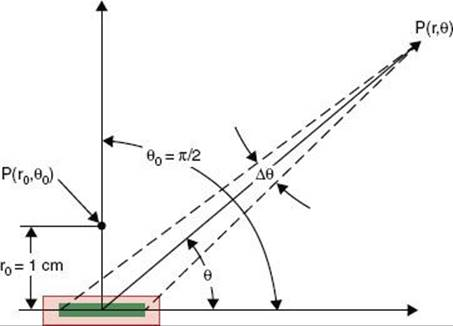
\includegraphics{figures/tg43.jpg}
\caption{TG 43}
\end{figure}

\textbf{Dose rate constant}

The \texttt{dose-rate\ constant} is defined as:

\begin{equation}
   \Lambda = \frac{\dot D(r_0, \theta_0)}{S_k}.
   \label{eq:dose-rate-constant}
\end{equation}

It can be thought as the dose rate in water at a reference point
(\(r_0\) = 1 cm for photon sources and 2 mm for beta emitters) along the
transverse axis (\(\theta = 90^{\circ }\)) for source strength of 1 U.

\textbf{Radial dose function and geometry function}

The \texttt{radial\ dose\ function} g(r) represents the attenuation of
radiation in tissue, defined as\\

\begin{equation}
g(r) = \frac{\dot D(r,90^{\circ})\cdot G(r_0,90^{\circ})}{\dot D(r_0,90^{\circ})\cdot G(r, 90^{\circ})}.
\end{equation}

where \(G(r,\theta)\) is the \texttt{geometry\ function} which accounts
for the effect of the distribution of radioactive material inside the
source on the dose distribution at a given point. It is equal to
\(1/r^2\) for point source approximation,
\(\frac{tan^{-1}[(x+L/2)/y]-tan^{-1}[(x-L/2)/y]}{Ly}\) or
\(\frac{1}{x^2-(L/2)^2}\) for linear source approximation with
\(\theta \neq 0^{\circ}\) or \(\theta = 0^{\circ}\) and \(x>L/2\).

\textbf{Anisotrpic function}

\(F(r,\theta)\) is the \texttt{anisotropy\ function}, defined as

\begin{equation}
F(r,\theta) = \frac{\dot D(r,\theta)\cdot G(r,90^{\circ})}{\dot D(r,90^{\circ})\cdot G(r, \theta)}.
\end{equation}

It accounts for anisotropy of dose distribution around the source,
including effects of absorption and scatter in medium, i.e.,
self-filtration in source, oblique filtration in walls, scattering and
absorption in tissue. In TG-43U, typically calculated from Monte Carlo.

The example information about Elekta Flexisource can be seen in the
figure below 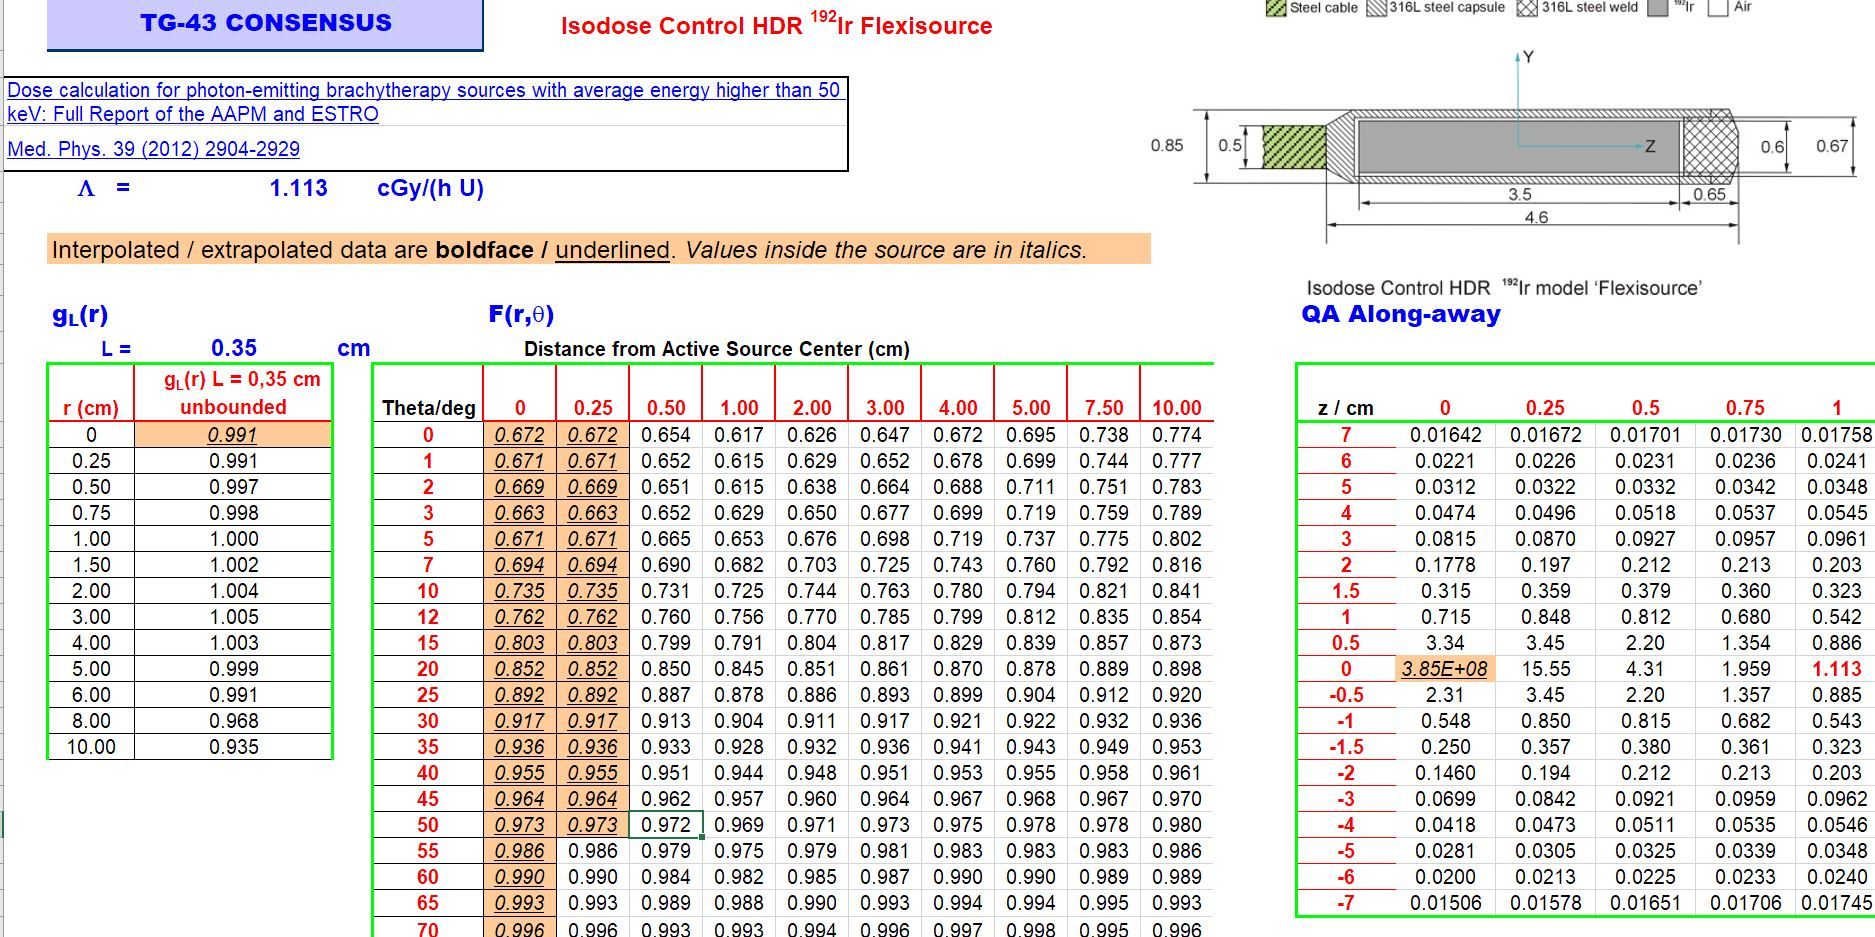
\includegraphics{figures/Ir-192.jpg}

In brachytherapy there is a rapid falloff in dose as distance from the
source increases due to inverse square law. The dose within the tumor
may much different from the prescription dose, thus the concept of
equivalent uniform dose (EUD) was introduced by Dale et al. (1997).
Mathematically, the generalized EUD is defined as

\begin{equation*}
EUD= \left( \sum \nu_iD^a_i \right ) ^{1/a}
\end{equation*}

Here \(\nu_i\) is the fractional organ volume receiving a dose \(D_i\)
and a is a tissue-specific parameter that describes the volume effect.

\begin{itemize}
\tightlist
\item
  \(a \rightarrow -\infty\), EUD = minimum dose;
\item
  \(a \rightarrow -\infty\), EUD = maximum dose (serial organs);
\item
  a = 1, EUD = mean dose;
\item
  a = 2, EUD = RMS dose.
\end{itemize}

The EUD model is parameterized by the single biological parameter a,
which should be chosen so that the EUD reflects the intended biological
properties for the given tumor or organ. Parameter a and the Lyman model
parameter n are related by a = 1/n Tumor: a is a negative number (e.g.,
a = -15) Normal tissues: a is a positive number

The volume-effect: very small normal tissue volumes (e.g.~1-2 cm3) can
tolerate very high doses that larger volumes would not tolerate. There
are a few exceptions to this such as spinal cord, though the dose as
high as 167.3 Gy to the cord has been reported in very low dose rate
brachytherapy of paraspinal tumor. Rogers et al. (2002) reported that
the mean cord dose was 72.5 Gy (ranging: 53.1-167.3 Gy), combining the
EBRT and I-125 brachytherapy.

\section{Solutions}\label{ldr-solutions}

\texttt{Q1\ d)}

As \(D = \dot D\times\Delta t\),
\(\frac{\Delta t_{new}}{\Delta t_{old}}=\frac{\dot D_{old}}{\dot D_{new}} = \frac{A_{old}}{A_{new}} = \frac{A_0e^{-10/30}}{A_0} = 0.79\)

\texttt{Q2\ Shielding\ b)}\\
Although the average energy of \textsuperscript{60}Co is higher than
that of \textsuperscript{226}Ra, there are gamma rays of 1.76 and 2.2
MeV emitted from \textsuperscript{226}Ra sources. In shielding design,
we need to consider their existence (although their contribution is
small) and thus HVL for \textsuperscript{226}Ra is greater than HVL for
\textsuperscript{60}Co.\footnote{\url{https://www.nrc.gov/docs/ML1122/ML11229A721.pdf}}\\
\texttt{Q3\ a)\ b)\ c)} A \textsuperscript{137}Cs source is normally
used for consistence check (like linac monthly QA) but not
calibration.\\
\texttt{Q4\ a)} Like external beam radiotherapy, the inverse square law
is always the biggest factor for dose calculation.\\
\texttt{Q5\ a)} Should c) and d) be correct?\\
\texttt{Q6\ Initial\ dose\ rate\ c)}

The prescription dose or total dose for an prostate implant is

\begin{equation*}
D = \int^{\infty}_0 \dot D_0 \cdot e^{-\frac{0.693}{T_{1/2}}t}dt
\end{equation*}

Using an important definite integral,
\(\int^{\infty}_0 e^{-ax} dx = \frac{1}{a}\), we can find that

\begin{equation*}
D = \dot D_0 \cdot \frac{T_{1/2}}{0.693} \rightarrow \dot D_0 = \frac{D}{59.4/0.693}=\frac{14400 \text{ cGy} \times 0.693}{59.4 \text{ days} \times 24 \text{ hours/day}} = \boxed{7.0\text{ cGy/hr}}
\end{equation*}

\texttt{Q7\ b)}

\texttt{Q8\ The\ Paterson-Parker\ system\ c)}\\
\texttt{Q9\ The\ Quimby\ system\ a)}\\
\texttt{Q10\ The\ Paris\ system\ c)\ d)}

The air kerma strength and \texttt{apparent\ activity} conversion is 1 U
= 0.348, 0.243, 0.486, 0.787, and 0.773 mCi for \textsuperscript{137}Cs,
\textsuperscript{192}Ir, \textsuperscript{198}Au,
\textsuperscript{125}I, and \textsuperscript{103}Pd, respectively.

\section{Traceability}\label{traceability}

Calibrations of brachytherapy sources should be directly traced to NIST
or to an Accredited Dosimetry Calibration Laboratory (ADCL) which is
traced to NIST. Normally, we don't send sources to NIST or ADCL, but
instead a well chamber with specific inserts designed for different
isotopes. To calibrate
\href{http://www.bardmedical.com/products/prostate-health/brachytherapy/source-and-delivery-systems/iodine-125/}{Bard~PS-1251L}
I-125 sources, for instance, the well chamber with an I-125 insert will
be used, which was checked using Bard PS-1251L I-125 sources at NIST or
ADLC.

TG-40

\begin{itemize}
\tightlist
\item
  all long half-life sources should be calibrated;
\item
  at least 10\% or 2 ribbons (whichever is larger) should be calibrated
  for a large number of loose seeds with \textbf{short} half-life.
\end{itemize}

If the institution's verification of source strength disagrees with the
manufacturer's data by more than 3\%, the source of the disagreement
should be investigated. We further recommend that an unresolved
disparity exceeding 5\% should be reported to the manufacturer.

Radioactive materials must be under control by the facility at all
times. This means under direct control or by securing in a locked area.

\chapter{Radiation Protection}\label{protection}

Historically, the most commonly used unit in US is millirem (mrem) where
rem stands for \emph{Roentgen Equivalent Man}. The SI unit of effective
dose and equivalent dose is \emph{Sievert} (Sv). Because 1 Sv, equal to
1 Gy numerically, is rather large quantity, the milliSievert (mSv) is
commonly used in practice. The relationship between mSv and mrem is
\[1\ mSv = 100\ mrem\].

\section{Sources of radiation
exposure}\label{sources-of-radiation-exposure}

According to the National Council on Radiation Protection and
Measurement (NCRP) report 160 (2009), the average annual radiation dose
per person in the U.S. is about 6.2 mSv, in which medical imaging
contributes about 50\% (e.g.~CT: 24\%, NM: 12\%, interventional
fluoroscopy 7\%, conventional radiography 5\%). Naturally occurring
sources of radiation include cosmic radiation (5\%), radioactive
minerals in the ground and in your body (5\%), and terrestrial radiation
emitted by naturally occurring materials such as uranium, thorium, and
radon (37\%) in earth. The pie chart of sources of radiation exposure
from NCRP 160 can be found
\href{https://19january2017snapshot.epa.gov/radiation/radiation-sources-and-doses_.html}{here}.

\begin{verbatim}
jdkhfakjdhfkljadsfdf
  
\end{verbatim}

\section{Stochastic and deterministic
event}\label{stochastic-and-deterministic-event}

Although the severity of the stochastic effect is independent of the
dose, the probability of having such effects is proportional to the dose
\textbf{without dose threshold}. The examples of stochastic effects
include radiation induced cancer and genetic mutation. Skin erythema,
epilation (hair loss), lens opacification, and tissue necrosis are best
described as non-stochastic or \textbf{deterministic} events. For
deterministic effects, there is a threshold and the severity of the
effect depends on the dose.

To avoid unacceptable complications, normal tissue should be below a
\textbf{tolerance dose} (TD) (Emami et al.) Complications is categorized
as fatal, severe (e.g.~grade 3-4 pneumonitis), and quality-of-life
complications. TD5\%/5 and TD50\%/5 are used to imply complications in 5
years.

Answer: e)

\section{TDS rule}\label{tds-rule}

Time (\(D \propto \dot{D}\times \Delta t\)), distance (inverse square
law), and shield (attenuation) measures are major factors in
consideration of minimizing the unavoidable radiation exposure. Other
procedures to minimize the exposure are containment and NRC's system for
radiation protection according to NRC guidelines. The NRC's system for
protection includes (1) dose limits for radiation workers and members of
the public; (2) monitoring and labeling radioactive materials; (3)
posting signs in and around radiation areas; and (4) reporting the theft
or loss of radioactive material. In addition, the NRC imposes penalties
for failures to follow the agency's regulations.

If the licensees' can limit the radiation to \textbf{1 mSv} to the
public and \textbf{50 mSv} to adult radiation works in a year, the NRC
may enter into an agreement with a State governor to give the State
authority for regulating radioactive materials. States that meet these
conditions and agree to regulate materials using the same standards as
the NRC are called \textbf{Agreement States}.

Answer: d)

\chapter{QA}\label{qa}

\href{https://vimeo.com/76862861}{Uncertainties in Radiation Medicine:
An Oncologist's Perspective}

CTV margin for subclinical tumor - ML

\href{https://aapm.onlinelibrary.wiley.com/doi/full/10.1120/jacmp.v16i3.5431}{Medical
physics practice guideline 4.a}

\chapter{TBI}\label{tbi}

\href{https://aapm.org/pubs/reports/RPT_17.pdf}{TG-17 (1986)} ``The
physical aspects of total and half body photon irradiation''

The reported D\_0\_ value - the amount of ionizing radiation necessary
to eradicate a particular cell type---of \emph{hematopoietic stem cells}
is 0.5 to 1.4 Gy, while those of human \emph{leukemia cell} lines are
0.8 to 1.5 Gy, indicating that both cells are radiosensitive.

Fractionated TBI has been shown to lead to a higher incidence of graft
rejection than the same dose delivered in a single fraction, possibly
due to DNA repair during interfraction intervals.4,7,12 However,
fractionation decreases the eradication of bone marrow stromal cells,
which are necessary for successful hematopoietic stem cell engraftment,
and is, therefore, considered the standard of treatment

\url{https://appliedradiationoncology.com/articles/total-body-irradiation-a-practical-review}

\url{https://www.ted.com/talks/daniel_kraft_invents_a_better_way_to_harvest_bone_marrow/transcript}

why TMR is SAD independent
\url{http://www.npl.co.uk/upload/pdf/20140513-dart-pres-byrne.pdf}

If only high-energy photons are available and superficial structures
would be underdosed,spoilers may be used. The ideal is to maintain a low
skin dose and increase dose in the build-up region, to emulate a lower
energy beam. However, while it is impossible to exactly mimic a lower
energy beam with a spoiler, the build-up characteristics may be
preferable to using bolus.

\chapter{Three-dimensional conformal radiotherapy}\label{crt}

\section{ICRU reference point}\label{icru-reference-point}

The ICRU reference point is the point in the center (or center parts) of
the PTV

\section{Image registration}\label{image-registration}

\begin{itemize}
\tightlist
\item
  Brady: Geometric (and Photometric) alignment of one image with another
  -- Images may be of same or different types (MR, CT, and etc.)
\item
  ITK: The process of determining the spatial transformation that maps
  points from one image to homologous points on an object in the second
  image.
\item
  Elastix: The task of finding a spatial one-to-one mapping from voxels
  in one image to voxels in the other image.
\end{itemize}

\section{Image segmentation}\label{image-segmentation}

\url{http://www.cs.uu.nl/docs/vakken/ibv/reader/chapter10.pdf}: the
division of an image into meaning structures. Wiki: image segmentation
is the process of partitioning a digital image into multiple segments
(sets of pixels) Khan: slice-by-slice delineation of targets and
organs-at-risk

\section{Cumulative DVH}\label{cumulative-dvh}

DVH See Chapter 11 Q6

\section{Differential DVH}\label{differential-dvh}

The choice of c): a certain dose within a specified dose interval as a
function of dose. The differential DVH is similar to conventional
histogram in statistics.

\chapter{IMRT}\label{imrt}

IMRT provides an ability to deliver many beamlets (smallest element to
be modified) of varying radiation density within one treatment field.

\section{IMRT}\label{imrt}

The number of photons was modulated by \textbf{blocking the photon
beams} (fluence) at specific location and/or time with MLC or
\textbf{changing the dose rate}\footnote{It is fancinating that how dose
  rates are changed in linacs. A 2013 PMB paper,
  \href{http://iopscience.iop.org/article/10.1088/0031-9155/58/4/1075/meta}{Radiobiological
  effects of altering dose rate in filter-free photon beams}, showed
  that altering radiotherapy dose rate through either changing pulse
  repetition frequency or instantaneous dose rate does \textbf{not} have
  an effect on cell survival. An increase in survival was seen in both
  modes upon protracting dose delivery to 15, 30 or 60 min rather than
  delivering acutely. \emph{Is this important to PLDR}? \emph{Should we
  increase the prescription dose}?}.

\section{Transmission or leakage}\label{transmission-or-leakage}

For current machines, In IMRT, the relative contribution to the target
dose from collimator transmission scatter is greatest for: a) leaf
transmission; b) round edge transmission; c) X-ray jaws; d) overall head
scatter Intra- and inter-leaf transmission: (Varian manual) Average
intra-leaf and maximum interleaf leakage for the Varian HD-120 MLC is
and 2.0\% and 2.5\% (up to 10 MV). Based on Bedford et al. (2013), the
maximum intra- and inter-leaf leakage for the Elekta Agility MLC (9 cm
height) is 0.5\% and 0.2\%. Leaf (round) end transmission is not
reported anymore, and should be in the range of 10\%-20\%. Jaw
transmission is about 1\% and 1.5\% for the Edge and Versa machine,
respectively.

\texttt{Q1:\ b),\ c)}

\section{Q4 MU: IMRT vs.~3DCRT}\label{q4-mu-imrt-vs.3dcrt}

Compared to the four-field box technique, an IMRT plan could require
\emph{substantially} more monitor units (MU). The MUs of an IMRT plan
largely depend on the degree of dose modulation within a target and/or a
proximity between a target and nearby OARs. With the improvement in
optimization algorithm and electro-mechanical performance of linac, the
difference of MUs between an IMRT plan (especially using VMAT technique)
and 3D-CRT plan has decreased.

\texttt{Q2:\ c}

\section{Q5}\label{q5}

In generating an intensity-modulated profile in minimum time with the
dynamic MLC: a) the opposing pair of leaves should move with equal but
variable speed; b)the leading leaf should move at the maximum speed and
trailing leaf should provide the required intensity modulation, if the
gradient of the intensity profile is positive (increasing fluence); c)
the trailing leaf should move at the maximum speed and trailing leaf
should provide the required intensity modulation, if the gradient of the
intensity profile is negative (increasing fluence); d) the two leaves
should move with equal and maximum speed, if the spatial gradient of the
intensity profile is zero.

\texttt{Q5:\ b),\ c),\ d)}

\section{Shielding for IMRT}\label{shielding-for-imrt}

If majority of the patients are to be treated with IMRT instead of
conventional radiation therapy, the total MUs will be largely increased
despite delivered dose remains the same. Therefore, the major concerns
would be the increased leakage radiation so is the design of the
secondary barrier. Solution: c and d

\section{}\label{section}

The difference between an IMRT and 3-D CRT delivery typically include:
a) Non-uniform (modulated) beam intensities; b) Patient-specific
beam-shaping c) Inverse planning for dose optimization; d) Dosimetric or
biological objectives with relative weights; e) Significantly more
complex dose calculation algorithm Solution: a c d

\section{Q8}\label{q8}

\begin{verbatim}
IMRT delivery technique include:
IMAT
Conformal arc therapy
Helical tomotherapy
DMLC delivery
SMLC delivery
\end{verbatim}

Solution: e

\section{Q9}\label{q9}

The term step-and-shoot is sometimes used to describe which IMRT
delivery technique: Helical tomotherapy Serial tomotherapy IMAT
Segmental MLC-IMRT Dynamic MLC-IMRT

\texttt{Q9:\ d)}

\section{Q10}\label{q10}

For a step-and-shoot IMRT treatment delivery, an MLC controller system
introduces 50 millisecond delay between the monitor chamber signal reach
a control point and beam termination. If the initial segment of a field
is set to receive 2 MU, what percent error does this delay introduce for
this segment if the linac's output is set to 600 MU/min? \textless{}1 5
10 25 250

\texttt{Q10:\ d)}

\section{MLC test(s)}\label{mlc-tests}

Which MLC test(s) are unique to dynamic MLC delivery? Linac performance
for small MU delivery Leaf positional accuracy Inter- and intra-leaf
leakage Tough-and-groove effect Leaf speed accuracy Solution: e

Generally speaking, the MLC delivery can be categorized into two types:
static (e.g., step-and-shoot) and dynamic (e.g., vmat and
conformal-arc). Linac performance on small MU delivery has been a
serious issue for static MLC delivery. Xia et al. (2002) has used a
simple formula to relate the dose error (\(\Delta\)) with dose rate (R),
communication time (T), and MU/segment (M): \(\Delta =RT/M\) For
example, if dose rate is 600 MU/min, T = 100 mS, and M = 1 MU/seg, the
dose error 1 or 100\%. Therefore, larger dose errors are expected for
smaller MU segments with certain dose rate and communication time.
Recent progress in increase of sampling rate (e.g., from 100 ms to 20
ms) and integration of MLC controller with the linac have significantly
improved the dose delivery accuracy for step-and-shoot IMRT Li et al.
(2012). In addition, as the optimization algorithms improved, the use of
increased minimal MU per segment (\textgreater{} 4-8) further reduce the
dose errors caused by smaller MU segments used in the plan. Leaf
positioning error impact also

\section{Q12}\label{q12}

The contribution of MLC leakage to the total dose from an IMRT field: Is
the largest contribution of the dose Increases with increase in leaf
speed Increases with increase in leaf gap width May be neglected in the
final dose calculation None of the above

Solution: e

More Inverse planning procedures Clinical objectives (goals) are
specified first in terms of desired (physical or biological ) dose or
DVH goals. Field's fluence map (the set of beamlet weights) is optimized
The optimize fluence is converted to deliverable MLC positions and
further optimization is continued It should be noted that the step 2 and
3 are integrated into the direct machine parameter optimization (DMPO).
Consideration of beam number and placement (shortest path to irradiate
targets and avoid OARs) Complexity of the target shape Proximity to
critical organs Collimator angle (minimize leakage and maximize
coverage)? Previous RT? Non-coplanar beams? Parallel opposed beams?

\chapter{SBRT}\label{sbrt}

\begin{quote}
The great difficulty in the world is not for people to accept new ideas,
but to make them forget about old ideas. -John Maynard Keynes
\end{quote}

\section{Milestones}\label{milestones}

\begin{itemize}
\tightlist
\item
  1908 Horsley and Clarke coined the term \texttt{stereotaxis} and
  fabricated an apparatus that can be rigidly clamped to the skull;
\item
  1947 Spiegel and Wycis frame\footnote{\texttt{Pneumoencephalography}
    is an painful procedure that requiring a spinal tap so that
    pressured air could be introduced into the cerebrospinal fluid
    space. This created two large air bubbles filling the patient's
    ventricles so that they could be imaged radiographically.
    (Interesting) the patient was suspended from the ceiling by a full
    body harness, which was rotated in 3D to assist the introduction of
    air into the brain. - Steven J. Goetsch ``Historic developement of
    SRS and SBRT'' in Stereotactic Radiosurgery and Stereotactic Body
    Radiation Therapy};
\item
  1949 Talairach defined anterior commissure - posterior commissure
  (AC-PC) line and a brain atlas;
\item
  1951 \href{https://en.wikipedia.org/wiki/Lars_Leksell}{Lars Leksell}
  developed a frame exclusively for human beings;\footnote{The location
    of the desired target was determined from radiographic procedure,
    and then translated to \texttt{Leksell\ coordinates}. The frame is
    still used for Gamma knife.}
\item
  1967 First SRS treatment on a Gamma Knife (GK) machine.
\item
  1991 Lax and Blomgren ``Extracranial sterotactic radiation therapy''
  at Karolinska.
\item
  1999 \href{https://www.ncbi.nlm.nih.gov/pubmed/10371630}{Adler et al.}
  IGRT-SRS on a Cyberknife (CK) machine.
\item
  2003 Timmerman Phase-I trial on lung cancer at Indiana U.
\item
  2005 SBRT CPT code added.
\item
  2018
  \href{https://www.cureus.com/articles/9924-self-shielding-analysis-of-the-zap-x-system}{ZAP
  system}
\end{itemize}

The SRS treatments have been delivered using GK, CK, tomotherapy
machine, and linear accelerators (Lutz \emph{et al.} (1987))\footnote{\href{https://www.ncbi.nlm.nih.gov/pubmed/3276655}{A
  system for stereotactic radiosurgery with a linear accelerator}.
  Extensive performance tests have shown that a target, localized by CT,
  can be irradiated with a positional accuracy of \textbf{2.4 mm} in any
  direction with 95\% confidence. This number has not been decreased
  much in last 30 years. The geometric accuracy of isocenter
  localization of \(\pm1\) mm is acceptable.}.

\section{The definition of SRS and
SBRT}\label{the-definition-of-srs-and-sbrt}

ACR/ASTRO definition of SBRT: an external beam radiation therapy method
used to very precisely deliver a high dose of radiation to an
extracranial target within the body, using either a single dose or a
small number of fractions.

To simulate the head frame used in the SRS, a body frame was used in
early SBRT treatments (Sweden and Japan) in early 1990s. With advances
of technologies, however, most current SBRT treatments do not use body
frames , because the localization accuracy is comparable between
frame-based and frameless SBRT and worse than that in the SRS.

\section{\texorpdfstring{Features of GAMMA Knife
Perfexion\textsuperscript{TM} and
Icon\textsuperscript{TM}}{Features of GAMMA Knife PerfexionTM and IconTM}}\label{features-of-gamma-knife-perfexiontm-and-icontm}

9/13/18 from GK manual

As part of the imaging process, it is essential to provide exact points
of reference by means of which the shape and position of the targets can
be ascertained with respect to the patient's skull. Moreover, during the
subsequent radiosurgery session, the head of the patient must be
entirely immobilized to maintain the accuracy of the shots.

\subsection{Stereotactic reference}\label{stereotactic-reference}

\begin{itemize}
\tightlist
\item
  use an indicator box during image acquisition
\item
  use the CBCT (only available for
  \href{https://www.youtube.com/watch?v=ZeFFwkxnoME}{Icon})
\end{itemize}

\subsection{Steps to create new plan}\label{steps-to-create-new-plan}

\begin{itemize}
\tightlist
\item
  Creat a new patient file

  \begin{itemize}
  \tightlist
  \item
    Have to complete the \textbf{Radiological Examination} field
  \end{itemize}
\item
  Plan \textbar{} New Plan to make a new treatment plan
\item
  Open a patient file Tomographic imaging acq
\end{itemize}

Leksell Coordinate System

\section{GK Troubleshooting}\label{gk-troubleshooting}

\begin{itemize}
\tightlist
\item
  \emph{When doing CBCT verification, the Frame docking did not work}

  \begin{itemize}
  \tightlist
  \item
    Ask engineering to fix the sensor which reads whether frame/mark
    dock is in position (\textbf{Docked}) and which frame is in position
    (\textbf{Docking}).
  \end{itemize}
\item
  \emph{The frame (one screw) became loose, what should be do?}

  \begin{itemize}
  \tightlist
  \item
    Tighten the screw, do an CBCT verfication scan
  \item
    Switch to mask case, you need to change \textbf{fixation} from frame
    to mask, and then do \textbf{Request CBCT - Stand}.
  \end{itemize}
\item
  \emph{If there are ``out of range'' warning messages when putting
  shots, what can you?}

  \begin{itemize}
  \tightlist
  \item
    to add measurement information and change gamma angle from
    90\textsuperscript{o} to 70\textsuperscript{o}.
  \end{itemize}
\end{itemize}

\textbf{Leksell Coordinate Frame G}
\href{https://www.youtube.com/watch?v=90vD3cxc9m0}{Gamma Knife
Perfexion} and

\begin{itemize}
\tightlist
\item
  The patient positioning system (\textbf{PPS}) is the treatment couch
\item
  A frame adapter attaches the Leksell coordinate frame (known geometry)
  to the treatment couch (known relative position to radiation
  isocenter)
\item
  Built-in collimation system, and 3 collimator size: 16, 8, and 4 mm
\item
  \textbf{192} Co-60 sources; (the model U, B, and C, still in use at
  some centers, have 201 sources.)
\item
  Souces are not fixed in space; they reside on 8 independent sectors
\item
  Each sector has 5 positions (4 mm, blocked, 8 mm, 16 mm, ?)
\end{itemize}

\section{QA of GK}\label{qa-of-gk}

\href{https://vimeo.com/88176011}{Paula Patti: QA for the Leksell Gamma
Knife Perfexion\textsuperscript{TM}}

Basic tests and measurements (following NRC licensing guidelines 10 CFR
35.1000)

\begin{enumerate}
\def\labelenumi{\arabic{enumi}.}
\tightlist
\item
  Coincidence of the \textbf{mechanical isocenter of the PPS} with
  radiation-focal point (or radiation isocenter, or unit center point)
\item
  Agreement of measured beam profiles with GK calculation for all
  collimator sizes in XY, YZ, and XZ planes
\item
  Measurement of the absolute dose rate calibration for largest
  collimator
\item
  Confirmation of the relative output factors for smaller collimators
\end{enumerate}

\subsection{Prescision and accuracy}\label{prescision-and-accuracy}

GK (radiation) isocenter: the center of the smallest sphere through
which all beam axes pass as the radiological
\texttt{Unit\ Center\ Point} (UCP) or isocenter. The radius of this
sphere may then be seen as a measure of the spread of the beam axes or
the uncertainty of their location. This uncertainty is called
\texttt{the\ precision\ of\ the\ Gamma\ Knife}.{[}\^{}Arndt
\href{https://www.aapm.org/meetings/99AM/pdf/2756-33420.pdf}{GK
Dosimetry and treatment planning}{]}

GK mechanical isocenter:

The mechanical accuracy of Gamma Knife radiosurgery based on
single‐isocenter measurement has been established to within 0.3 mm.

The following radiophysical data is pre-stored in Gamma Plan:

\begin{itemize}
\tightlist
\item
  4 beam profiles (OARs), one for each beam sizes measured at
  \textbf{400 mm} distance from source center and at 80 mm depth in
  polystyrene.
\item
  One data set to analytically calculate Percentage Depth Dose (PDD)
\item
  4 measured output factors, one for each beam size
\end{itemize}

\section{Commissioning of GK}\label{commissioning-of-gk}

The ion chamber is widely used for the measurement of the depth dose in
conventional photon beams. The correction for the depth dose measurement
depends on the ratio of the mass attenuation coefficient of the detector
material and water, \(\left( \mu/\rho \right )^{detector}_{water}\). In
another word, if the detector is near tissue (water) equivalent, i.e.,
near equivalent Z number, there is no necessity for depth correction.
Although silicon diodes and radiographic films typically need
corrections, the diamond diodes (unlike silicon diodes) and radiochromic
films are both near tissue-equivalent.

\section{Preparation of GK Treatment
Planning}\label{preparation-of-gk-treatment-planning}

\subsection{Frame Application: model C}\label{frame-application-model-c}

The Leksell frame runs from 40 mm to 160 mm in the X axis using the
automatic positioning system (\textbf{APS}), runs from 25 mm to 175 mm
in the Y axis, and the Z axis values are not marked on the frame but are
calculated by the treatment planning software from fiducial markers.

\subsection{Frame application:
Perfexion}\label{frame-application-perfexion}

With the Perfexion model a new instrument has been introduced called the
\textbf{frame cap}. Special care is needed if a lesion is very posterior
or very anterior.

\section{GK Plan Indices}\label{gk-plan-indices}

\subsection{Systematic Errors}\label{systematic-errors}

Based on the rule for sums and differences in error propagation,

\begin{equation*}
\varepsilon_{total}=\sqrt{\varepsilon_{x}^{2}+\varepsilon_{y}^{2}+\varepsilon_{z}^{2}}
\end{equation*}

\section{Linac-based SRS}\label{linac-based-srs}

\subsection{Cone-based}\label{cone-based}

For linac SRS systems, the fields are mostly shaped by tertiary cone
collimation system. The tertiary cones are precisely machined, closer to
patient (smaller geometric penumbra), and diverging beam shaping further
minimizes penumbra (see
\href{http://www.aapm.org/meetings/amos2/pdf/59-17160-8941-53.pdf}{Yenice
(2011) AAPM presentation}, page2).

\begin{itemize}
\tightlist
\item
  Smith \emph{et al.} (1993)
  \href{http://onlinelibrary.wiley.com/doi/10.1002/roi.2970010111/full}{Role
  of Tertiary Collimation for Linac-Based Radiosurgery}. They found that
  the geometrical penumbra (how they separate dosimetric and geometrical
  penumbra?) of tertiary cone for \textbf{2 mm focal spot} in only
  \textbf{0.6 mm}, which is much smaller than 5.1 mm and 3.3 mm from the
  upper and lower jaw.
\item
  Novotny \emph{et al.} (2008)
  \href{http://thejns.org/doi/pdf/10.3171/JNS/2008/109/12/S3}{Dosimetric
  comparison between the GK Perfexion and 4C}. They found good agreement
  between dosimetric parameters of those two models for 4- and 8-mm
  collimators.
\item
  Wen \emph{et al.} (2015)
  \href{http://onlinelibrary.wiley.com/doi/10.1120/jacmp.v16i4.5313/pdf}{Characteristics
  of a novel treatment system for linac-based SRS}. They found that the
  penumbra is about 1.2-1.8 mm for 6FFF and 2.3-5.1 mm for 10 FFF beams
  (80\%-20\%).
\end{itemize}

\section{Diesease sites treatment with
SRS}\label{diesease-sites-treatment-with-srs}

Commonly treated tumors using the SRS technique include:

\subsection{Acoustic neuoromas}\label{acoustic-neuoromas}

\subsection{Arteriovenous malforamtions
(AVM)}\label{arteriovenous-malforamtions-avm}

\subsection{Brain metastases}\label{brain-metastases}

\subsection{Malignant gliomas}\label{malignant-gliomas}

\subsection{Menningiomas}\label{menningiomas}

Keeping the margin dose \textgreater{} 12 Gy seems to be effective

?? Much of the current assessment of control rates is based on Kaplan
Meier statistics rather than raw data. In the future there will be more
raw data to give a more reliable assessment.

\subsection{Pituitary tumors}\label{pituitary-tumors}

\subsection{Unilateral Vestibular
Schwannomas}\label{unilateral-vestibular-schwannomas}

Using \textbf{12-13 Gy} with a noticeable improvement in the rate of
complications, particular hearing loss (pay attention to cochlear nerve)
and facial .

\subsection{Uveal melanomas}\label{uveal-melanomas}

One of the odd features of this tumours is its well known ability to
prove deadly from systemic metastases, years after an enucleation of an
affected eye; metastases usually in the liver. Where the metastases
reside in the interval is not known.

Interesting treatment technique: fix the eye motion; check the positions
in the dose plan against physical measurements using polymer gel with MR
images.

\subsection{Trigeminal neuralgia}\label{trigeminal-neuralgia}

The recommended doses can be found
\href{http://www.aboutcancer.com/gk_doses.htm}{here}. The dose typically
depends on the tumor size (the smaller the tumor, the higher the
prescription dose).

\texttt{a)\ wrong;\ c)\ wrong;\ Rhabdomyosarcoma\ is\ mostly\ treated\ with\ linac.}

\section{Dose fall-off}\label{dose-fall-off}

Currently higher X-ray, \(\gamma\)-ray, and protons are used to treat
SRS/SRT.

\texttt{a);\ d)}

SRS treatment are characterized by steep dose gradients, for example,
\textgreater{}50\%/cm, at the target periphery. If the spatial accuracy
of the treatment delivery is \(\pm\) 1 mm, the dosimetric uncertainty in
this region will be \textgreater{}50\%/cm times 1 mm, which equals to
\textgreater{}5\%/cm.

\texttt{d)}

\texttt{b);\ c)}

\section{Required measurements for commissioning a SRS/SBRT
program}\label{required-measurements-for-commissioning-a-srssbrt-program}

The measurements required for commissioning a SRS/SRT program are
similar to conventional external beam radiotherapy with the exception of
transmission measurement which is typically very small due to the
construction of the cone collimator.

\texttt{a);\ c);\ d)}

\texttt{b)\ is\ wrong\ as\ the\ average\ energy\ from\ Co-60\ sources\ is\ 1.25\ MeV\ not\ 6\ MV;\ c)\ is\ wrong\ because\ sources\ move\ in\ the\ translational\ mode;\ d)\ is\ wrong\ because\ the\ Gamma\ knife\ is\ more\ accurate\ than\ a\ linac-based\ SRS\ system.}

\href{https://link.springer.com/article/10.1007/s00701-014-2275-6}{Mindermann
(2015) Gamma Knife, CyberKnife or micro-multileaf collimator LINAC for
intracranial radiosurgery?}, is a good read. The author questioned a few
dosimetric studies in comparing several delivery systems, and stated
that the questions of dosimetry needs to be answered, which include: the
source of the photon radiation (cobalt-60 or linear accelerator); the
nature of the collimators (fixed aperture, iris, micro-multileaf, etc.);
moving or stationary radiation sources during beam-off time or beam-on
time; the fixation of the head; the planning software; the imagery used;
the way the images are acquired (dedicated protocols, head fixation,
etc.); the number of beams; the number of arrival angles; the exit dose;
the scatter factor of a given beam; the distance source to target; the
time period over which a dose is delivered; the system's overall
accuracy; dose rates; the nature and the size of the lesion; the shape
of the lesion; its proximity to organs at risk; the experience and the
neurosurgical and anatomical knowhow of the radiosurgeon.

SBRT prostate using spacer
\href{https://www.spaceoar.com/physicians/clinical-publications/}{spaceoar.com}

\chapter{HDR}\label{hdr}

\section{HDR vs.~LDR}\label{hdr-vs.ldr}

LDR: well-established treatment; standard doses, plan, and treatmetn
time\footnote{\begin{itemize}
  \tightlist
  \item
    \href{https://www.ncbi.nlm.nih.gov/pubmed/16874815}{Current
    controversies in high-dose-rate versus low-dose-rate brachytherapy
    for cervical cancer}.
  \item
    \href{https://www.aapm.org/education/vl/vl.asp?id=3911\%5D}{Showalter
    2014 AAPM}
  \end{itemize}}\\
HDR: Outpatient treatment, short administration time, minimal staff
exposure, standard source strength, and dose optimization

\section{Common indications in
practice}\label{common-indications-in-practice}

\begin{itemize}
\tightlist
\item
  GYN (cervical\footnote{\href{http://cochranelibrary-wiley.com/doi/10.1002/14651858.CD007563.pub2/abstract}{Cochrane
    review} and its
    \href{https://www.ncbi.nlm.nih.gov/m/pubmed/25300170/?i=5\&from=/10432431/related}{update}:
    there is no difference in OS, DSS, LC, nodal occurrence, distance
    occurrence was found between LDR and HDR (from a meta-analysis of 4
    clinical trials in \emph{Cochrane database} with a total of 1265
    patients with advanced cervical cancer), but HDR is more convenient
    and accurate.}, uterine, vaginal, vulvar)
\item
  Prostate (monotherapy or boost)
\item
  Breast (accelerated partial breast irradiation)
\item
  possible Sarcoma, skin, esophagus, and bile duct
\end{itemize}

?? Theoretically, HDR has a lower therapeutic ratio than LDR because of
the short duration of the treatments. How? - Practical ROP chapter
``Intracavitary Brachytherapy''

\section{HDR-QA}\label{hdr-qa}

\subsection{Daily QA}\label{daily-qa}

According
\href{https://www.nrc.gov/reading-rm/doc-collections/cfr/part035/part035-0643.html}{10~CFR35.643},
the AMP needs to review the daily QA within \textbf{15 days}.

\subsection{Pretreatment QA (TG-59)}\label{pretreatment-qa-tg-59}

\begin{enumerate}
\def\labelenumi{\arabic{enumi}.}
\tightlist
\item
  Two people (therapists?) should check proper \textbf{connection of
  catheters} to the HDR unit and that the transfer tubes are free of
  kinks.
\item
  The emergency kit and source container are available.
\item
  Survey meter and/or GM-counter is present and operational. (The
  patient may have had a nuclear medicine scan prior to the treatment,
  causing an elevated reading. thus a \textbf{pre-treatment survey} is
  conducted though not listed in TG-59).
\item
  The \textbf{length} of transfer tube and applicator (catheters) are
  correct.
\item
  Check applicator positioning. How do physicians check this item
  without image verification?
\item
  Treatment documentation review.

  \begin{enumerate}
  \def\labelenumii{\alph{enumii}.}
  \tightlist
  \item
    Signed prescription and plan.
  \item
    Second check has been performed. (use emipircal values)
  \item
    Plan agrees with prescription.
  \item
    Plan is consistent with previous fractions if applicable.
  \item
    Dwell positions and times in plan agree with what is programmed on
    the treatment console.
  \end{enumerate}
\item
  Patient identity confirmed by two methods.
\end{enumerate}

At current practice, a \textbf{check-list} is used by physicists for
pretrement plan QA and a time-out is conducted prior to initiating the
treatment.

\subsection{Source change}\label{hdr-source-change}

The half-life time is about 74 days, so the old source is sawpped with a
new source about every 3 months. The activity of the new source is
normally about \textbf{10 Ci}. According to Eq. \eqref{eq:sk} and Eq.
\eqref{eq:exposure}, it is equal to 41100 U
(\(S_k = 10,000\ (mCi) \times 4.69 \left(\frac{{R\cdot cm}^2}{mCi\cdot hr} \right) \times 0.876 \left(\frac{cGy}{R}\right)\)).
This quantity will be verified by an autheried medical physicist
(\textbf{AMP}) using NIST tracable well chamber and electrometer, and
then enterred in the treatment planning system for dose calculation. The
engineering from HDR afterloader vendor also verifies the source using
their own equipment.

\begin{enumerate}
\def\labelenumi{\arabic{enumi}.}
\tightlist
\item
  Verify the source cable \textbf{positioning accuracy} at two different
  programmed positions (1205 mm and 1400 mm) before the vendor
  engineering leaves (using GYN transfer tube).
\item
  Although the well chamber and electrometer is still within 2-year
  calibration period, we always do \textbf{consistence check} using a
  NIST-traceble Cs-137 source (we actually checked with 2 Cs-137 sources
  provided by our RSO).
\item
  Switch a physics QA transfer tube and insert a catheter into Ir-192
  insert.
\item
  Measure current at 5 positions (1195 mm, 1200 mm, 1205 mm, 1210 mm,
  and 1215 mm) and take an average
\item
  Check time-dose linearity
\item
  Check stopwatch accuracy (100 s)
\item
  Check transfer tube connection error
\item
  Switch emergency power switch
\item
  Check
\end{enumerate}

\section{Medical Events}\label{medical-events}

\begin{itemize}
\tightlist
\item
  \href{http://www.nrc.gov/reading-rm/doccollections/nuregs/brochures/br0117/}{Errors
  on NRC website}
\item
  \href{(http://chapter.aapm.org/GLC/media/2011/tollenaar.pdf)}{Wisconsin}
\end{itemize}

\section{Source}\label{source}

A comprehensive seed data source can be found from a
\href{http://www.physics.carleton.ca/clrp/seed_database}{database}
provided by Carleton University

Because
\href{https://www.estro.org/about/governance-organisation/committees-activities/tg43-ir-192-hdr}{Ir-192}
has much higher \texttt{special\ activity} than most other isotopes, it
is now the mostly used radio-isotope for HDR treatment. The higher the
special activity means that the Ir-192 can be made with small physial
dimension but still provide high radioactivity.

The special activity (SA) is defined as the activity per mass. It
depends on half lifetime and atomic number,
\(SA \propto \frac{1}{T_{1/2}\cdot A}\). For example,
\(\frac{SA_{Co}}{SA_{Ir}} = \frac{74\ days \times 192}{5\ years \times 60} \approx 0.13\).
Wait a second, how about SA of I-125? Although I-125 can have higher SA
than Ir-192, the energy of I-125 is just too low for enough tissue
penetration.

Co-60 has been used recently!

\section{Treatment sites}\label{treatment-sites-1}

\subsection{Endometrial cancer}\label{endometrial-cancer}

\href{https://www.sciencedirect.com/science/article/pii/S1538472111003874?via\%3Dihub}{ABS
consensus guidelines for adjuvant vaginal cuff brachytherapy after
hysterectomy}

\begin{itemize}
\tightlist
\item
  Dose fractionation: 7Gy \(\times\) 3 prescribed to 0.5 cm is a common
  fractionation scheme with active length of 5 cm
  (\(\color{Purple} {\text{Are we treating vaginal cuff or the whole vigina?}}\))
\item
  the standard applicator is a segmented cylinder with one central
  catheter; the \textbf{largest diameter} cylinder that patient can
  tolerate is used to minimize the air gap between cylinder and vagina
  and to avoid rapid dose fall-off.
\end{itemize}

\subsection{Cervical cancer}\label{cervical}

\begin{itemize}
\tightlist
\item
  \href{}{ABS consensus guidelines for locally advanced carcinoma of the
  cervix. Part I: General principles}
\item
  \href{https://www.sciencedirect.com/science/article/pii/S1538472111003515}{ABS
  consensus guidelines for locally advanced carcinoma of the cervix.
  Part II: High-dose-rate brachytherapy}
\end{itemize}

Cervical cancer is mostly treated with HDR brachytherapy.

\begin{itemize}
\tightlist
\item
  1903 Stockholm and Paris
\item
  1938 Manchester -- point A
\item
  1953 Point A revision
\item
  1985 ICRU 38
\item
  1987 more point A updates
\item
  2000 GEC-ESTRO

  \begin{itemize}
  \tightlist
  \item
    D90, D100 for dose prescription
  \item
    D2cc bladder, rectum, and sigmoid
  \end{itemize}
\item
  2004 GTV and CTV delineation (MRI)
\item
  2005 GEC-ESTRO recommendation for IGRT brachytherapy
\end{itemize}

\begin{quote}
Improvement occurred only in tumours \textgreater{}5 cm: OS 28\% versus
58\% (p = 0.003) - R. Potter (2007) in ``Clinical impact of MRI assisted
dose volume adaptation and dose escalation in brachytherapy of locally
advanced cervix cancer''.
\end{quote}

\textbf{GEC-ESTRO target volumes}\footnote{Schwarz 2015 AAPM Spring
  Clinical Meeting ``Defining Targets for Brachytherapy''
  \url{https://www.aapm.org/education/vl/vl.asp?id=4077}}

\begin{itemize}
\tightlist
\item
  \texttt{Gross\ tumor\ volume\ (diagnosis)} (GTV\textsubscript{D})

  \begin{itemize}
  \tightlist
  \item
    \textbf{macroscopic} tumor extension at diagnosis
  \item
    detected by clinical examination and as visualized on MRI (high
    signal intensity mass(es) at \emph{fast spine echo} (FSE) sequences
    T2 in cervix/corpus, parametria, vagina, bladder, and rectum)
  \end{itemize}
\item
  \texttt{Gross\ tumor\ volume\ (brachy)} (GTV\textsubscript{B1},
  GTV\textsubscript{B2}, \ldots{})

  \begin{itemize}
  \tightlist
  \item
    \textbf{macroscopic} tumor volume at time of brachy
  \item
    detected by clinical examination and as visualized on MRI
  \end{itemize}
\item
  \texttt{High\ risk\ CTV} (HR CTV\textsubscript{B1}, HR
  CTV\textsubscript{B2}, \ldots{})

  \begin{itemize}
  \tightlist
  \item
    includes GTV\textsubscript{Bx} and the whole cervix or MRI grey
    zones?
  \item
    represent \textbf{macroscopic} tumor load
  \end{itemize}
\item
  \texttt{Intermediate\ risk\ CTV} (IR CTV\textsubscript{B1}, IR
  CTV\textsubscript{B2}, \ldots{})

  \begin{itemize}
  \tightlist
  \item
    areas with a significant \textbf{microscopic disease}
  \item
    IR CTV = HR CTV + 5-15 mm margin for limited diseases
  \item
    based on GTV\textsubscript{D} for extensive disease
  \end{itemize}
\end{itemize}

\textbf{Applicator imaging}

\textbf{Idea}: availability of commercial dummy sources for MRI is
limited.

Based on GEC-ESTRO recommendations\footnote{\href{https://www.sciencedirect.com/science/article/pii/S0167814010003683}{Recommendations
  from Gynaecological (GYN) GEC-ESTRO Working Group: Considerations and
  pitfalls in commissioning and applicator reconstruction in 3D
  image-based treatment planning of cervix cancer brachytherapy}}, the
choice of MR sequence is essential for optimal visualisation of the
applicator. There are difference between plastic and titanium
applicators\footnote{Haack et al 2009 Applicator reconstruction in MRI
  3D image-based dose planning of brachytherapy for cervical cancer.
  \url{https://doi.org/10.1016/j.radonc.2008.09.002}}

\begin{itemize}
\tightlist
\item
  Plastic has weak signal on T2; use of markers
\item
  Titanium has (induced) susceptibility artifact, and thus more
  distortions for higher magnetic strength; worse on T2; T1 is more
  suitable (? Why Titanium is MR compatible? )
\item
  If an applicator has been shown to be MR conditional for a 1.5T MRI,
  then it does \textbf{not} mean that it can be safely used in a 3T
  system without the need for further testing. CT still provides best
  imaging for applicator in terms of spatial accuracy (1 mm on CT
  vs.~1-2 mm on MRI for the localization of first dwell position) and
  artifacts.
\end{itemize}

\textbf{Prescription Dose}

\begin{itemize}
\tightlist
\item
  HDR prescription: 5.5 Gy \(\times\) 5, 6 Gy \(\times\) 5, or 7 Gy
  \(\times\) 4; once a week
\item
  HR CTV: total dose \textgreater{} 85 Gy \textbf{Can we go higher? or
  fewer fractions}
\item
  IR CTV: 60 Gy
\end{itemize}

\subsection{Breast}\label{breast}

ABS acceptability criteria for APBI

\begin{itemize}
\tightlist
\item
  Age: \(\ge\) 50 year old
\item
  Size: \(\le\) 3 cm
\item
  Histology: All invasive subtypes and DCIS
\item
  Estrogen receptor: +/-
\item
  Surgical margin: -
\item
  Lymphovasucular space invasion: not present
\item
  Nodal status: -
\end{itemize}

Treatment planning

\begin{itemize}
\tightlist
\item
  34 Gy in 10 fractions twice daily
\item
  PTV\textsubscript{Eval} + D90\% \textgreater{}= 90\% + V150
  \textless{} 50 cm\textsuperscript{3} + V200 \textless{} 10
  cm\textsuperscript{3} + Skin dose \textless{} 145\% of prescription
\end{itemize}

They are slightly different from ASTRO Consensus Statement 2009.

\subsection{Prostate}\label{prostate}

\href{https://www.sciencedirect.com/science/article/pii/S1538472111004004}{ABS
consensus guidelines for high-dose-rate prostate brachytherapy}

Monotherapy: 13.5 Gy \(\times\) 2 fractions (NCCN)

\section{References}\label{references}

\begin{itemize}
\tightlist
\item
  \href{https://www.aapm.org/pubs/reports/rpt_41.pdf}{TG-41 (1993)}
  Remote Afterloading Technology.
\item
  \href{https://www.aapm.org/pubs/reports/detail.asp?docid=50}{TG-43
  (1995)} Dosimetry of Interstitial Brachytherapy Sources.
\item
  TG-43U (2004) A revised AAPM protocol for brachytherapy dose
  calculations.
\item
  \href{https://www.aapm.org/pubs/reports/detail.asp?docid=58\#}{TG-56
  (1997)} Code of practice for brachytherapy physics.
\item
  \href{https://pdfs.semanticscholar.org/5a32/c14e0720d3e5af0747e5a191845683b3feca.pdf}{TG-59
  (1998)} High dose-rate brachytherapy treatment delivery.
\item
  \href{https://www.aapm.org/pubs/reports/detail.asp?docid=167}{AAPM
  UN-25 (2017)} Supplement 2 for the 2004 update of the AAPM Task Group
  No. 43 Report: Joint recommendations by the AAPM and GEC-ESTRO.
\item
  ABS guideline:
  \url{https://www.americanbrachytherapy.org/guidelines/cervical_cancer_taskgroup.pdf}.
\item
  Damato AL, Lee LJ, Bhagwat MS, et al. Redesign of process map to
  increase efficiency: Reducing procedure time in cervical cancer
  brachytherapy. Brachytherapy. 2015;14:471--480.
\item
  Dose Optimization in Gynecological 3D Image Based Interstitial
  Brachytherapy using Martinez Universal Perineal Interstitial Template
  (MUPIT) -An Institutional Experience. J Med Phys (2014) 39 (3):
  197-202.
\item
  Kim et al., ``Evaluation of artifacts and distortions of titanium
  applicators on 3.0-Tesla MRI: Feasibility of titanium applicators in
  MRI-guided brachytherapy for gynecological cancer,'' Int J Radiation
  Oncology, 80 (3), 947-55 (2011).
\end{itemize}

\section{Solutions}\label{solutions-1}

\textbf{Q1 Dose rate} c)\\
\textbf{Q2} a)\\
\textbf{Q3 TG43U } d)

Using Eq. @ref(eq.tg43) or TG-43U1 2D Brachytherapy dosimetry formalism,

\begin{equation}
\begin{aligned}
   \dot D(r, \theta) &= \Lambda\cdot S_k \frac{G_L(r, \theta)}{G_L(r=1cm,\theta=90^o)} \cdot g_L(r, \theta)\cdot F(r,\theta)\\
   &=1.12\ cGy/(h\cdot U)\cdot4.11\times10^4\text{U}\cdot1.023\cdot1\\
   &=\boxed{13.1\ cGy/s}
\end{aligned}
\end{equation}

\textbf{Q4 Afterloader QA} a)\\
\textbf{Q5 Shiedling} b)\\
\textbf{Q6 Impact of decay on treatment timee}

The half-life time of Ir-192 is about 74 days, so activity after 90 days
(Eq. (\eqref{eq:decay2})) is

\begin{equation*}
    A_2 = A_02^{-t/T_{1/2}}=A_02^{-90/74}=0.43A_1
\end{equation*}

To maintain the prescribed dose
(\(\dot D_1 \Delta t_1 = \dot D_2 \Delta t_2\) and \(A \propto \dot D\),
the dwell time \(\Delta t_2\) will be

\begin{equation*} 
{\Delta t_2 = \frac{\dot D_1}{\dot D_2} \Delta t_1 = \frac{\dot A_1}{\dot A_2} \Delta t_1 = \frac{1}{0.43}\times 16 \text{ min} \ \times 80\% = \boxed{29.7 \text{ min}}}
\end{equation*}

The total treatment time will be
\(29.7 + 16\times20\%=\boxed{33\ \text{minutes}}\).

\textbf{Q7} c)\\
\textbf{Q8} c)\\
\textbf{Q9} b) \textbf{Q10} a) but esophagus cancer is also treated with
HDR but with less indication`\\
\textbf{Q11} b)\\
\textbf{Q12} d)

\chapter{Implants}\label{implants}

\section{Isotopes}\label{isotopes-1}

good reference
(\url{https://aapm.org/meetings/amos2/pdf/42-11873-3201-79.pdf})

\begin{longtable}[]{@{}lllll@{}}
\toprule
Isotope & \(T_{1/2}\) (days) & Median E (KeV) & 90\% dose delivered
(days) & Rx (Gy)\tabularnewline
\midrule
\endhead
I-125 & 60 & 28 & 204 & 145\tabularnewline
Pd-103 & 17 & 22 & 58 & 120 or 125\tabularnewline
Cs-131 & 10 & 29 & 33 & 115\tabularnewline
Y90 & 2.67 & 937 & 11 & 120-150\tabularnewline
\bottomrule
\end{longtable}

\begin{equation}
  \dot D(r, \theta) = \Lambda S_k \frac{G(r,\theta)}{G(1,\pi/2)} g(r) F(r,\theta)
\end{equation}

where

\begin{itemize}
\tightlist
\item
  \(\dot D(r,\theta)\) is the dose rate at point P in a medium
\item
  \(\Lambda\) is the dose rate constant
\item
  \(S_k\) is the air kerma strength of the source
\item
  G is the geometry factor
\item
  g is the radial dose function
\item
  F is the anisotropy function
\end{itemize}

\section[Patient Release]{\texorpdfstring{Patient Release\footnote{Wendt
  2013 AAPM \url{https://www.aapm.org/education/VL/vl.asp?id=2439}}}{Patient Release}}\label{patient-release}

\href{https://www.nrc.gov/reading-rm/doc-collections/nuregs/staff/sr1556/}{NRC-NUREG-1556}
in Table U.1

\begin{longtable}[]{@{}lllll@{}}
\toprule
\begin{minipage}[b]{0.13\columnwidth}\raggedright\strut
Isotope\strut
\end{minipage} & \begin{minipage}[b]{0.13\columnwidth}\raggedright\strut
Activity threshold (GBq)\strut
\end{minipage} & \begin{minipage}[b]{0.13\columnwidth}\raggedright\strut
Activity threshold (mCi)\strut
\end{minipage} & \begin{minipage}[b]{0.13\columnwidth}\raggedright\strut
Dose rate at 1 m (mSv/hr)\strut
\end{minipage} & \begin{minipage}[b]{0.13\columnwidth}\raggedright\strut
Dose rate at 1 m (mrem/hr)\strut
\end{minipage}\tabularnewline
\midrule
\endhead
\begin{minipage}[t]{0.13\columnwidth}\raggedright\strut
I-125\strut
\end{minipage} & \begin{minipage}[t]{0.13\columnwidth}\raggedright\strut
0.33\strut
\end{minipage} & \begin{minipage}[t]{0.13\columnwidth}\raggedright\strut
9\strut
\end{minipage} & \begin{minipage}[t]{0.13\columnwidth}\raggedright\strut
0.01\strut
\end{minipage} & \begin{minipage}[t]{0.13\columnwidth}\raggedright\strut
\textbf{1}\strut
\end{minipage}\tabularnewline
\begin{minipage}[t]{0.13\columnwidth}\raggedright\strut
Pd-103\strut
\end{minipage} & \begin{minipage}[t]{0.13\columnwidth}\raggedright\strut
1.5\strut
\end{minipage} & \begin{minipage}[t]{0.13\columnwidth}\raggedright\strut
40\strut
\end{minipage} & \begin{minipage}[t]{0.13\columnwidth}\raggedright\strut
0.03\strut
\end{minipage} & \begin{minipage}[t]{0.13\columnwidth}\raggedright\strut
\textbf{3}\strut
\end{minipage}\tabularnewline
\begin{minipage}[t]{0.13\columnwidth}\raggedright\strut
\ldots{}\strut
\end{minipage} & \begin{minipage}[t]{0.13\columnwidth}\raggedright\strut
\ldots{}\strut
\end{minipage} & \begin{minipage}[t]{0.13\columnwidth}\raggedright\strut
\ldots{}\strut
\end{minipage} & \begin{minipage}[t]{0.13\columnwidth}\raggedright\strut
\ldots{}\strut
\end{minipage} & \begin{minipage}[t]{0.13\columnwidth}\raggedright\strut
\ldots{}\strut
\end{minipage}\tabularnewline
\begin{minipage}[t]{0.13\columnwidth}\raggedright\strut
Y90\strut
\end{minipage} & \begin{minipage}[t]{0.13\columnwidth}\raggedright\strut
NA\strut
\end{minipage} & \begin{minipage}[t]{0.13\columnwidth}\raggedright\strut
NA\strut
\end{minipage} & \begin{minipage}[t]{0.13\columnwidth}\raggedright\strut
NA\strut
\end{minipage} & \begin{minipage}[t]{0.13\columnwidth}\raggedright\strut
NA\strut
\end{minipage}\tabularnewline
\begin{minipage}[t]{0.13\columnwidth}\raggedright\strut
Tc-99m\strut
\end{minipage} & \begin{minipage}[t]{0.13\columnwidth}\raggedright\strut
28\strut
\end{minipage} & \begin{minipage}[t]{0.13\columnwidth}\raggedright\strut
760\strut
\end{minipage} & \begin{minipage}[t]{0.13\columnwidth}\raggedright\strut
0.58\strut
\end{minipage} & \begin{minipage}[t]{0.13\columnwidth}\raggedright\strut
\(\color{red} {58}\)\strut
\end{minipage}\tabularnewline
\bottomrule
\end{longtable}

1 mR/hr = 1 mrem/hr for gamma and x-ray

The activity at which patients could be released was calculated by
using, the method discussed in the NCRP Report No. 37, ``Precautions in
the Management of Patients Who Have Received Therapeutic Amounts of
Radionuclides.''

\begin{equation}
  D(t)=34.6\times \frac {\Gamma Q_0 T_P \left(1-e^{-0.693/T_P}\right)}   {r^2},
\end{equation}

where

\begin{itemize}
\tightlist
\item
  34.6 = Conversion factor of 24 hrs/day times the total integration of
  decay (1.44)
\item
  D(t) = accumulated exposure at time t, in R (It assumed that \textbf{1
  R = 10 mSv = 1 rem})
\item
  \(\Gamma\) = Specific gamma ray constant for a point source, R/mCi-hr
  at 1 cm
\item
  \(Q_0\) = Initial activity of the point source in mCi, at the time of
  the release
\item
  \(T_P\) = Physical half-life in days
\item
  r = Distance from the point source to the point of interest, in cm
\item
  t = Exposure time in days
\end{itemize}

\section{Prostate implants}\label{prostate-implants}

Good Pre-Plan (Seattle Prostate Institute Criteria)

\begin{itemize}
\tightlist
\item
  \emph{Modified uniform loading}
\item
  V100: 98-100\%
\item
  V150:

  \begin{itemize}
  \tightlist
  \item
    I-125: 30-40\%
  \item
    Pd-103: 40-50\%
  \end{itemize}
\item
  V200: 10-20\%
\item
  Uretha max: 100-125\% (definitely\textless{}150\%)
\item
  Rectum point: \textless{}80\%
\item
  Margin: 3-5 mm
\end{itemize}

\section{TheraSphere}\label{y90}

\textsuperscript{90}Y-microsphere therapy usually target the liver,
taking advantage of the unique circulatory system in the liver Portal
vein (normal liver) and hepatic artery (tumor).\footnote{\url{http://amos3.aapm.org/abstracts/pdf/68-19792-237349-87867.pdf}}

SIR-Sphere is not discussed here but more detailed descriptions about
both microsphere can be found from 2017 AAPM Annual meeting talk,
\emph{\textsuperscript{90}Y-Microsphere Therapy: Emerging Trends and
Future Directions}
\href{https://www.aapm.org/education/vl/vl.asp?id=12296}{(link)}.

Patient selection (an example)

\begin{itemize}
\tightlist
\item
  62 year-old female with cirrhosis and HCC
\item
  BSA = 1.78
\item
  Child-pugh B
\item
  UNOS T3
\item
  ECOG perfomance status = 1 (Fatigue)
\item
  AFP 809
\end{itemize}

Before treatment

To avoid radiation pnumanitis, the lung dose for TheraSphere should be
less than \textbf{30 Gy}. The \emph{lung shunt} (LS) percentage can be
calculated from the signals (counts) in Tc-99m (normally 2-4 mCi) MAA
planar scintigraphy or SPECT/CT\footnote{why we need CT? similar to the
  function of CT in PET/CT?},

\begin{equation}
  lung\ shunt\ (\%) = \frac{Lung\ Counts}{Lung\ Counts+Liver\ Counts}\times 100
  \label{eq:ls}
\end{equation}

where \(GM counts= \sqrt{ANT{count}\times POST{count}}\).

Delineation of target volumes is based on
\texttt{digital\ segmentated\ angiography} - DSA, CT, C-arm CBCT,
SPECT/CT. The treatment volume is then converted to mass, using a
conversion facotr of 1.03 g/cc. The required activity can then be
calculated

\textbf{Standard model}

\[ A_{Totoal} = A_{Liver} + A_{Lung}\]

\begin{equation}
  D_{Lung} = \frac {50 (\text{J}/\text{GBq})\times A_{Lung}\times LSF} {M_{Lung}}. 
  \label{eq:y90-lung}
\end{equation}

\begin{equation}
  D_{Liver} = \frac {50 (\text{J}/\text{GBq})\times A_{Lung}\times (1-LSF)} {M_{Liver}}. 
  \label{eq:y90-liver}
\end{equation}

Issues of the standard model

\begin{itemize}
\tightlist
\item
  Hetergeneous uptake distribution
\item
  unknow Tumor dose and normal tissue dose
\end{itemize}

\textbf{Partiion model}

After treatment

Typical patient exposure rates

\begin{itemize}
\tightlist
\item
  Maximum surface: 5 - 25 mR/hr
\item
  At 1 m: 0.1 - 0.3 mR/hr
\end{itemize}

Residual measurement at 30 cm on a template.

The radioactive \textsuperscript{90}Y-label microspheres (20-30
\(\mu m\)) are injected via a catheter trans-aterially.

d d c d \emph{a} b

\chapter{Intravascular BT}\label{ivbt}

We have finished a nice book.

\chapter{IGRT}\label{igrt}

\textbf{References}

TG-76 (2006) The management of respiratory motion in Radiation Oncology

Several publications about QA issues associated with image-guided
radiation therapy

\begin{itemize}
\tightlist
\item
  TG-58 (2001) Clinical use of electronic portal imaging

  \begin{itemize}
  \tightlist
  \item
    Planar MV
  \end{itemize}
\item
  TG-142 (2009): QA of medical accelerators

  \begin{itemize}
  \tightlist
  \item
    planar kV and MV; kV- and MV-CBCT
  \end{itemize}
\item
  TG-104 (2009): The Role of In-Room kV X-Ray Imaging for Patient setup
  and Target Localization

  \begin{itemize}
  \tightlist
  \item
    Planar kV and kV-CBCT
  \end{itemize}
\item
  TG-148 (2010) QA for helical Tomotherapy

  \begin{itemize}
  \tightlist
  \item
    Fan beam MVCT
  \end{itemize}
\item
  TG-154 (2011) QA of US-guided External beam radiotherapy for prostate
  cancer
\item
  TG-135 (2011): QA for Robotic Radiosurgry

  \begin{itemize}
  \tightlist
  \item
    planar kV
  \end{itemize}
\item
  TG-179 (2012): QA for image-guided radiation therapy utilizing
  CT-based technologies

  \begin{itemize}
  \tightlist
  \item
    kV- and MV-CBCT; fan beam kVCT and MVCT 
  \end{itemize}
\item
  TG-147 (2012): QA for nonradiographic RT localization and positioning
  systems
\item
  Jaffrey (2012) Assuring safety and quality in image-guided delivery of
  RT
\end{itemize}

\chapter{Cyber Knife}\label{cyber-knife}

A linear accelerator in CyberKnife generates a 6 MV x-ray beam. The
microwave frequency it uses for accelerating electrons is in the range
of: a) 500 to 1,000 MHz b) 2 to 4 GHz c) 8 to 12 GHz d) 15-20 GHz

\chapter{Proton RT}\label{proton}

We have finished a nice book.

\url{https://stackoverflow.com/questions/36293511/creating-custom-blocks-in-rstudios-bookdown}

\chapter{Information Technology}\label{it}

\section{IT basics}\label{it-basics}

\href{https://www.aapm.org/pubs/reports/detail.asp?docid=142}{AAPM
TG-201 - Information technology resource management in radiation
oncology (2009)}

\begin{figure}

{\centering 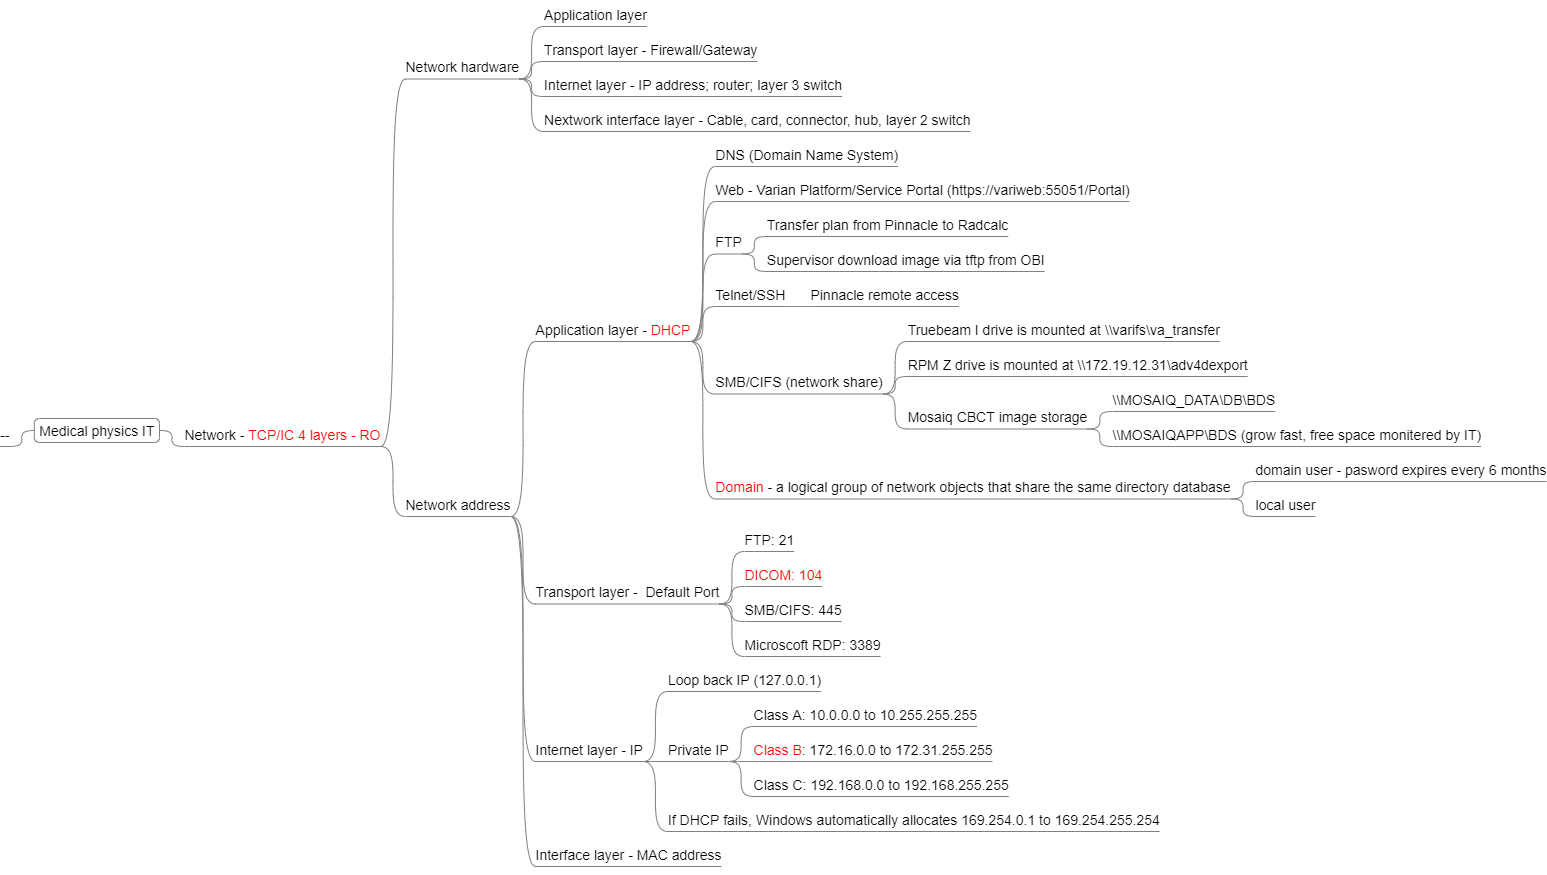
\includegraphics{figures/mp_it} 

}

\caption{Medical physics IT}\label{fig:it}
\end{figure}

\section{DICOM}\label{dicom}

\section{Database basics}\label{database-basics}

\section{Programming}\label{programming}

\bibliography{book.bib,packages.bib}


\end{document}
